% Options for packages loaded elsewhere
\PassOptionsToPackage{unicode}{hyperref}
\PassOptionsToPackage{hyphens}{url}
\PassOptionsToPackage{dvipsnames,svgnames,x11names}{xcolor}
\documentclass[
  british,
  10pt,
  a4paper,
]{article}
\usepackage{xcolor}
\usepackage[margin=22mm]{geometry}
\usepackage{amsmath,amssymb}
\setcounter{secnumdepth}{-\maxdimen} % remove section numbering
\usepackage{iftex}
\ifPDFTeX
  \usepackage[T1]{fontenc}
  \usepackage[utf8]{inputenc}
  \usepackage{textcomp} % provide euro and other symbols
\else % if luatex or xetex
  \usepackage{unicode-math} % this also loads fontspec
  \defaultfontfeatures{Scale=MatchLowercase}
  \defaultfontfeatures[\rmfamily]{Ligatures=TeX,Scale=1}
\fi
\usepackage{lmodern}
\ifPDFTeX\else
  % xetex/luatex font selection
  \setmainfont[]{DejaVu Serif}
  \setsansfont[]{DejaVu Sans}
  \setmonofont[]{DejaVu Sans Mono}
  \setmathfont[]{DejaVu Math TeX Gyre}
\fi
% Use upquote if available, for straight quotes in verbatim environments
\IfFileExists{upquote.sty}{\usepackage{upquote}}{}
\IfFileExists{microtype.sty}{% use microtype if available
  \usepackage[]{microtype}
  \UseMicrotypeSet[protrusion]{basicmath} % disable protrusion for tt fonts
}{}
\usepackage{setspace}
\makeatletter
\@ifundefined{KOMAClassName}{% if non-KOMA class
  \IfFileExists{parskip.sty}{%
    \usepackage{parskip}
  }{% else
    \setlength{\parindent}{0pt}
    \setlength{\parskip}{6pt plus 2pt minus 1pt}}
}{% if KOMA class
  \KOMAoptions{parskip=half}}
\makeatother
\usepackage{longtable,booktabs,array}
\newcounter{none} % for unnumbered tables
\usepackage{calc} % for calculating minipage widths
% Correct order of tables after \paragraph or \subparagraph
\usepackage{etoolbox}
\makeatletter
\patchcmd\longtable{\par}{\if@noskipsec\mbox{}\fi\par}{}{}
\makeatother
% Allow footnotes in longtable head/foot
\IfFileExists{footnotehyper.sty}{\usepackage{footnotehyper}}{\usepackage{footnote}}
\makesavenoteenv{longtable}
\usepackage{graphicx}
\makeatletter
\newsavebox\pandoc@box
\newcommand*\pandocbounded[1]{% scales image to fit in text height/width
  \sbox\pandoc@box{#1}%
  \Gscale@div\@tempa{\textheight}{\dimexpr\ht\pandoc@box+\dp\pandoc@box\relax}%
  \Gscale@div\@tempb{\linewidth}{\wd\pandoc@box}%
  \ifdim\@tempb\p@<\@tempa\p@\let\@tempa\@tempb\fi% select the smaller of both
  \ifdim\@tempa\p@<\p@\scalebox{\@tempa}{\usebox\pandoc@box}%
  \else\usebox{\pandoc@box}%
  \fi%
}
% Set default figure placement to htbp
\def\fps@figure{htbp}
\makeatother
\ifLuaTeX
\usepackage[bidi=basic,shorthands=off]{babel}
\else
\usepackage[bidi=default,shorthands=off]{babel}
\fi
\ifPDFTeX
\else
\babelfont{rm}[]{DejaVu Serif}
\fi
\ifLuaTeX
  \usepackage{selnolig} % disable illegal ligatures
\fi
\setlength{\emergencystretch}{3em} % prevent overfull lines
\providecommand{\tightlist}{%
  \setlength{\itemsep}{0pt}\setlength{\parskip}{0pt}}

\usepackage{xcolor}
\definecolor{reportteal}{HTML}{087F8C}
\definecolor{reportink}{HTML}{26323D}
\usepackage{xurl}
\urlstyle{tt}
\usepackage{fvextra}
\RecustomVerbatimEnvironment{Verbatim}{Verbatim}{breaklines=true,breakanywhere=true,fontsize=\small}
\usepackage{etoolbox}
\AtBeginEnvironment{longtable}{\footnotesize\setlength{\tabcolsep}{4pt}\renewcommand{\arraystretch}{1.18}}
\usepackage{titlesec}
\titleformat{\section}{\Large\bfseries\raggedright\color{reportteal}}{}{0em}{}
\titleformat{\subsection}{\large\bfseries\raggedright\color{reportink}}{}{0em}{}
\titleformat{\subsubsection}{\normalsize\bfseries\color{reportink}}{}{0em}{}
\titlespacing*{\section}{0pt}{2.0ex plus .8ex}{1.0ex}
\titlespacing*{\subsection}{0pt}{2.0ex plus .6ex}{.8ex}
\usepackage{fancyhdr}
\pagestyle{fancy}
\fancyhf{}
\fancyhead[L]{\small\color{reportink}Spectral optimizer investigation}
\fancyhead[R]{\small 7 September 2026}
\fancyfoot[C]{\small\thepage}
\setlength{\headheight}{15pt}
\renewcommand{\headrulewidth}{.3pt}
\setlength{\emergencystretch}{5em}
\tolerance=3000
\setlength{\parskip}{.5em}
\setlength{\parindent}{0pt}
\setcounter{tocdepth}{2}
\AtBeginDocument{\hypersetup{breaklinks=true,linkcolor=reportteal,urlcolor=reportteal,citecolor=reportteal}}
\makeatletter
\renewcommand{\maketitle}{%
  \hypersetup{pageanchor=false}%
  \begin{titlepage}\thispagestyle{empty}
  \vspace*{1.2cm}
  {\large\sffamily\color{reportteal}CURRENT SYNTHESIS AND MATHEMATICAL FOLLOW-UP\par}
  \vspace{1.0cm}
  {\Huge\bfseries\color{reportink}\@title\par}
  \vspace{.8cm}
  {\Large Cross-repository mathematical and empirical investigation\par}
  \vspace{1.0cm}
  {\large\@author\par}
  \vspace{.35cm}
  {\large\@date\par}
  \vfill
  {\normalsize Integrated findings from the cross-repository investigation and six
  completed continuations, with mathematical derivations, contradictory
  evidence, ranked hypotheses and discriminating tests.\par}
  \vspace{.7cm}
  {\small Source-derived companion artifacts remain in the investigation
  directory. The PDF preserves their citations; it does not embed the raw
  experiment arrays or the original private correspondence.\par}
  \vspace*{.8cm}
  \end{titlepage}%
  \hypersetup{pageanchor=true}%
}
\makeatother
\usepackage{bookmark}
\IfFileExists{xurl.sty}{\usepackage{xurl}}{} % add URL line breaks if available
\urlstyle{same}
\hypersetup{
  pdftitle={What the spectral optimizer does},
  pdfauthor={Codex --- Spectral Optimizer Investigation},
  pdflang={en-GB},
  colorlinks=true,
  linkcolor={Maroon},
  filecolor={Maroon},
  citecolor={Blue},
  urlcolor={Blue},
  pdfcreator={LaTeX via pandoc}}

\title{What the spectral optimizer does}
\author{Codex --- Spectral Optimizer Investigation}
\date{Current synthesis · 7 September 2026}

\begin{document}
\maketitle

{
\setcounter{tocdepth}{2}
\tableofcontents
}
\setstretch{1.08}
\clearpage

\section*{Reading this edition}\label{reading-this-edition}
\addcontentsline{toc}{section}{Reading this edition}

This edition integrates the cross-\allowbreak{}repository
investigatio\allowbreak{}n,\allowbreak{} completed continuation
experiments 001--006, and reviewed mathematical
follow-\allowbreak{}ups.\allowbreak{} The synthesis is the current
argument; two appendices preserve more detailed derivations and their
assumptions.\allowbreak{} The original report delivered on 6 September
is preserved separately.\allowbreak{}

The strongest empirical conclusion is task-\allowbreak{}dependent
suppression of late label memorization\allowbreak{}.\allowbreak{}
Directional regularization with Adam mediation is the leading
provisional explanation,\allowbreak{} not a demonstrated universal
denoising mechanism. Contradictory results and unrun tests remain
explicit.

This document is a research checkpoint,\allowbreak{} not completion of
the ongoing goal. No experiment is currently running at the report cut:
the iteration 007 preparation attempt failed without a new scientific
result.

Raw results, scripts, review records and the earlier evidence book
remain linked companion artifacts. They are not embedded in this PDF;
local file links require the repository.\allowbreak{} Internal links to
the two included mathematical reports work within this PDF. The build
manifest hashes the three embedded Markdown sources, figures, build code
and generated outputs.

\clearpage

\section{Synthesis}\label{synthesis}

\subsection{Executive summary}\label{synthesis--executive-summary}

Confidence is high that the optimizer is a
\textbf{history-\allowbreak{}dependent,\allowbreak{}
task-\allowbreak{}dependent directional regularizer whose delivered
gradient is subsequently transformed by AdamW}; confidence is only
moderate in this as the dominant causal account. It learns a low-rank
space of recent \emph{centered gradient variation}, then filters the raw
current gradient. It is not, by construction\allowbreak{},\allowbreak{}
a detector of clean labels, semantic signal, persistent signed
agreement, Hessian curvature, or the useful part of a gradient.

The central contradiction is immediate: hard rank-32 versus AdamW at
each method's validation-\allowbreak{}accuracy-\allowbreak{}selected
checkpoint is \textbf{−2.38 points in I4 but +4.827 points in I6},
across different three-seed bundles. The strongest stable result is
instead late anti-\allowbreak{}memorization\allowbreak{}.\allowbreak{}
The historical three-seed noisy-\allowbreak{}MNIST comparison has a
42.\allowbreak{}52-\allowbreak{}point final advantage, but only 1.69
points at each method's test-\allowbreak{}selected peak. The evidence
supports suppression of late fitting, not universal improvement in
attainable performance or replacement of ordinary early stopping.

The continuations sharpen rather than dissolve that
conclusion.\allowbreak{} Wider covariance storage clearly reduces
truncation-\allowbreak{}induced adaptation delay on a synthetic switch
and tracks a finite-\allowbreak{}history rank-32 reference more
faithfully on common neural gradient streams. Neither result establishes
better learning. In endogenous filtered training, widening sometimes
helps accuracy and sometimes hurts; its measured
clean-\allowbreak{}minus-\allowbreak{}corruption retention advantage is
small and inconsistent\allowbreak{}.\allowbreak{} A scalar
gradient-\allowbreak{}norm control does not reproduce the endpoint
preservation\allowbreak{},\allowbreak{} but it also does not match the
resulting AdamW step. Current-\allowbreak{}observation
self-\allowbreak{}inclusion is geometrically large, yet lagging the
basis does not reliably help: it harms clean performance in both tested
seed bundles, while the noisy effect reverses sign between the primary
and fresh bundles.

Cross-\allowbreak{}repository outcomes impose strong boundary
conditions.\allowbreak{} Clean CIFAR can underfit;
sparse-\allowbreak{}parity grokking slows while
modular-\allowbreak{}addition grokking speeds; a
near-\allowbreak{}clean-\allowbreak{}accuracy-\allowbreak{}matched CIFAR
robustness recipe is worse on every tested radius in the arm means; the
final Numerai spectral candidate transfers poorly to later eras amid
major recipe confounds; and
emergent-\allowbreak{}misalignment\allowbreak{} results do not isolate a
general safety benefit. Noise can itself be
low-\allowbreak{}dimensional,\allowbreak{} structured,\allowbreak{}
curvature-\allowbreak{}aligned,\allowbreak{} or temporally
persistent.\allowbreak{}

The leading scientific hypothesis is therefore learned directional
regularizati\allowbreak{}on,\allowbreak{} with Adam history and
coordinatewise normalization as a likely material mediator. Confidence
is high in the algebraic distinctions\allowbreak{},\allowbreak{}
moderate in this broad account, and low in any uniquely identified
causal mechanism. The highest-\allowbreak{}value next evidence is not
another broad performance sweep: it is
complete-\allowbreak{}state,\allowbreak{} same-batch one-step
measurement of raw versus filtered AdamW displacements and independent
clean, fixed-\allowbreak{}corruption and soft-\allowbreak{}target probe
losses, followed by independent-\allowbreak{}batch diagnostics that
separate conditional batch variability from mean surprise.

No experiment is currently running. Iteration 007's one-shot CPU
preparation failed with main-\allowbreak{}process exit 2 and produced no
scientific measurement; the consumed failure is preserved. Replacement
would require explicit new scope. The optimizer, defaults, original 6
September Markdown/\allowbreak{}PDF,\allowbreak{} and broader continuing
investigation remain unchanged.

\subsection{Abstract}\label{synthesis--abstract}

This report integrates the reconstructed
implementati\allowbreak{}on,\allowbreak{} classical
experiments,\allowbreak{} cross-\allowbreak{}repository
applications\allowbreak{},\allowbreak{} six focused
continuation\allowbreak{}s,\allowbreak{} and the 7 September
mathematical analyses of the spectral optimizer. The canonical method
maintains a recursively truncated covariance sketch of centered temporal
gradient innovations,\allowbreak{} uses its leading space to filter the
raw current gradient, and then relies on AdamW for the parameter update.
This construction selects high recent variation, not useful information
by definition.\allowbreak{} Replicated noisy-\allowbreak{}label
experiments show substantial preservation of late clean accuracy, but
clean underfitting\allowbreak{},\allowbreak{}
task-\allowbreak{}dependent grokking, negative
adversarial-\allowbreak{}robustness results, weak temporal transfer in
the final Numerai comparison,\allowbreak{} and unresolved language-
model behavior studies rule out a general denoising
interpretati\allowbreak{}on.\allowbreak{} Newer controlled evidence
further separates endpoints from selected checkpoints,\allowbreak{}
covariance fidelity from utility, and projected gradients from actual
updates. In particular,\allowbreak{} the sign of the
validation-\allowbreak{}accuracy-\allowbreak{}selected
noisy-\allowbreak{}MNIST effect against AdamW reverses between two
three-seed bundles, and lagged-\allowbreak{}basis effects on noisy data
reverse between a primary and fresh bundle. Conditional covariance
identities,\allowbreak{} fixed-\allowbreak{}Jacobian analysis, and
label-\allowbreak{}noise geometry support a more qualified account: the
filter changes which local function directions remain easy to learn,
while Adam can rotate and rescale the
intervention\allowbreak{}.\allowbreak{} The leading hypothesis is
task-\allowbreak{}dependent directional regularization with unresolved
Adam mediation. Concrete same-state tests are specified to distinguish
it from simple restraint, covariance-\allowbreak{}tracking,\allowbreak{}
truncation,\allowbreak{} and self-\allowbreak{}inclusion accounts.

\subsection{\texorpdfstring{1. Scope, provenance,\allowbreak{} and
evidence
levels}{1. Scope,  and evidence levels}}\label{synthesis--scope-provenance-and-evidence-levels}

This is a bounded synthesis of evidence already present in the
repository and the audited cross-\allowbreak{}repository
investigatio\allowbreak{}n.\allowbreak{} It adds no training run,
raw-data reanalysis,\allowbreak{} external search, optimizer
modification\allowbreak{},\allowbreak{} or new default. The
\href{../../../research/spectral_optimizer_investigation_2026-09-06.md}{original
6 September investigation} remains the detailed reconstruction of
repositories\allowbreak{},\allowbreak{} worktrees, reports, emails, code
and experiment history. The \href{../audit/final-resolution.md}{final
review resolution} records the corrections accepted after independent
review. In particular,\allowbreak{} the production Numerai spectral
refits used constant learning rate rather than a completed cosine
schedule; the configured schedule horizon was inert.

Source priority is committed code and raw metrics; focused reports tied
to those artifacts; maintained synthesis; then planning notes and
recollection\allowbreak{}.\allowbreak{} Numerical claims link to the
closest focused report or raw result. The original inventory covered 391
current classical JSON paths and 36 archive-\allowbreak{}only paths, but
these are coverage counts, not independent
replications\allowbreak{}.\allowbreak{}

Four evidence labels are useful:

\begin{itemize}
\tightlist
\item
  \textbf{Established} means an implementation fact, exact
  derivation,\allowbreak{} audited
  reconstructi\allowbreak{}on,\allowbreak{} or empirical pattern
  replicated across relevant seeds or settings.
\item
  \textbf{Supported} means direct evidence exists but is limited to a
  small number of seeds, one task, one model, or a selected recipe.
\item
  \textbf{Provisional} means a mechanism or generalization is compatible
  with the record but has not survived a discriminating
  intervention\allowbreak{}.\allowbreak{}
\item
  \textbf{Historical or invalid for the stronger claim} preserves
  provenance without treating old, confounded,\allowbreak{} malformed,
  or superseded evidence as confirmation\allowbreak{}.\allowbreak{}
\end{itemize}

The six focused continuations are not six independent confirmations of
one effect. Iterations 001 and 002 are controlled mechanism examples;
003, 004 and 006 are small MNIST policy studies with different paired
seed bundles; 005 is a passive replay on the iteration-\allowbreak{}004
AdamW streams. Repeated checkpoints and probe observations are dependent
within trajectories\allowbreak{}.\allowbreak{} Test accuracy from the
same official MNIST test set does not become new independent evidence
each time a checkpoint is evaluated.

\subsection{2. The algorithm---and the spectral objects it is
not}\label{synthesis--the-algorithmand-the-spectral-objects-it-is-not}

Let \(g_t\in\mathbb R^p\) be the flattened batch gradient and β the
decay. The canonical filter updates an exponential mean and forms a
centered innovation.\allowbreak{} For an idealized regular update with
rank truncation,\allowbreak{} the covariance recurrence is:

\[
m_t=\beta m_{t-1}+(1-\beta)g_t,\qquad
c_t=g_t-m_t=\beta(g_t-m_{t-1}),
\]

\[
C_t=\mathcal T_r\!\left[\beta C_{t-1}
 +(1-\beta)c_tc_t^T\right],\qquad P_t=V_tV_t^T.
\]

Here \(P_t\) is idealized as an
orthoproject\allowbreak{}or.\allowbreak{} The native
finite-\allowbreak{}precision action is \(V_t(V_t^Tg_t)\), which need
not be an exact orthoprojector; startup, residual rejection, pruning and
repair also qualify the displayed recurrence.\allowbreak{} After warmup,
hard mode delivers \(h_t=P_tg_t\) in this ideal notation. The current
raw gradient is used to update the basis before that same gradient is
projected: the observer is self-\allowbreak{}inclusive.\allowbreak{} The
covariance state is represented by
\(V_t\operatorname{diag}(S_t^2)V_t^T\), avoiding a dense \(p\times p\)
matrix. The stable code uses an orthonormal augmented basis, a small
float64 symmetric eigensolve,\allowbreak{} scale-\allowbreak{}aware
rejection, reorthogonalization and periodic repair. These improve
numerical geometry; they do not turn recursive truncation into exact PCA
of the complete history. The source of record is the
\href{../../../spectral_filter.py}{canonical filter}, with
reconstruction and executable counterexamples in the
\href{../analysis/mathematical-audit.md}{mathematical audit}.

Startup and memory matter. The first nonzero innovation initializes with
\(c_jc_j^T\), not \((1-\beta)c_jc_j^T\); at β=.99 this initially gives
that innovation 100 times an ordinary observation's covariance weight.
Repeated rank truncation creates a distinct hysteresis: evidence for a
new weak direction can be discarded at every step before it accumulates
enough mass to displace an incumbent mode. Storage and projection are
\(O(pr)\), but rotating the basis and solving the reduced eigenproblem
introduce \(O(pr^2)\) and \(O(r^3)\) work.

The name ``spectral'' covers at least four different objects in this
research history, and conclusions do not transfer automatically among
them:

{\def\LTcaptype{none} % do not increment counter
\begin{longtable}[]{@{}
  >{\raggedright\arraybackslash}p{(\linewidth - 4\tabcolsep) * \real{0.3333}}
  >{\raggedright\arraybackslash}p{(\linewidth - 4\tabcolsep) * \real{0.3333}}
  >{\raggedright\arraybackslash}p{(\linewidth - 4\tabcolsep) * \real{0.3333}}@{}}
\toprule\noalign{}
\begin{minipage}[b]{\linewidth}\raggedright
Spectral object
\end{minipage} & \begin{minipage}[b]{\linewidth}\raggedright
Space and statistic
\end{minipage} & \begin{minipage}[b]{\linewidth}\raggedright
Intervention
\end{minipage} \\
\midrule\noalign{}
\endhead
\bottomrule\noalign{}
\endlastfoot
Per-\allowbreak{}example gradient Gram matrix & Sample or microbatch
similarity at one model state & Reweight examples or project a mean
through a sample-\allowbreak{}space eigensystem \\
Temporal covariance of flattened gradients &
Parameter-\allowbreak{}space variation across training observations &
Filter the current gradient through a learned historical basis \\
Singular spectrum of one matrix gradient or momentum & Row/column
geometry within a layer & Matrix
precondition\allowbreak{}ing,\allowbreak{} polar update, or low-rank
coordinate compression \\
Singular spectrum of a LoRA/\allowbreak{}effective weight change &
Geometry of accumulated parameter change & Describe or regularize the
trained adapter \\
\end{longtable}
}

The canonical optimizer is the second. “Per-\allowbreak{}matrix” means
separate temporal covariance sketches for vectorized weight matrices; it
is not an SVD filter of the current matrix gradient. LoRA rank,
covariance storage rank, delivered projection rank and effective adapter
rank are different quantities.\allowbreak{} The older normalized
sample-\allowbreak{}space consensus algorithm is different again: its
eigenvectors come from row-\allowbreak{}normalized example gradients
while its update uses raw rows.

Soft mode is also qualitatively different from hard
projection.\allowbreak{} With residual enabled, tracked directions
receive weights \(w_i=(\lambda_i/\lambda_{\max})^\alpha\), while the
untracked complement remains at weight one, followed by
raw-\allowbreak{}gradient norm restoration.\allowbreak{} Increasing α
thus suppresses weak \emph{tracked} modes while preserving the
complement; it does not converge to a single leading direction. Without
residual, α=0 gives a norm-\allowbreak{}restored hard
projection,\allowbreak{} not the unnormalized hard method. Results from
these variants must keep their intervention labels.

Most importantly,\allowbreak{} the projector constrains AdamW's input,
not necessarily its parameter displacement\allowbreak{}.\allowbreak{}
Coordinatewise adaptive scaling does not generally preserve a rotated
subspace, momentum carries previous directions,\allowbreak{} and weight
decay adds another component. Therefore ``projected gradient,'' ``step
in the subspace,'' ``matched gradient norm,'' and ``matched
parameter-\allowbreak{}step norm'' are not synonyms.

\subsection{\texorpdfstring{3. What the cross-\allowbreak{}repository
outcomes
establish}{3. What the  outcomes establish}}\label{synthesis--what-the-cross-repository-outcomes-establish}

\subsubsection{\texorpdfstring{3.1 Random-\allowbreak{}label
anti-\allowbreak{}memorization\allowbreak{} is real but
conditional}{3.1   is real but conditional}}\label{synthesis--random-label-anti-memorization-is-real-but-conditional}

The strongest positive evidence is that selected hard temporal filters
can prevent large losses of clean accuracy late in training on randomly
relabelled MNIST and CIFAR. In the historical three-seed MNIST run at
nominal 90\% replacement,\allowbreak{} Adam ended at 37.22\% mean
clean-test accuracy and legacy global hard rank 200 at 79.74\%, a
42.\allowbreak{}52-\allowbreak{}point endpoint difference.\allowbreak{}
Their test-\allowbreak{}selected peaks were 83.19\% and 84.88\%, only
1.69 points apart. A fixed random projector ended at 56.03\%, and the
LoRA control at 31.94\%. These values and seed curves are recorded in
the \href{../analysis/classical-evidence.md}{classical evidence ledger}.

The stable one-seed 60-epoch comparison gives AdamW .3893, global
rank-200 .7877 and per-matrix rank-64 .8174 clean-test accuracy, with
179.40 MiB versus 57.41 MiB basis storage for the two spectral layouts.
The matrix rank was chosen on a scout using that seed, so this is
supporting evidence, not an unbiased
global-\allowbreak{}versus-\allowbreak{}matrix estimate; see the
\href{../../../results/noisy_mnist_hard_curves/summary.json}{raw
summary}.

Nominal 90\% uniform replacement does not mean 90\% wrong labels. With
ten classes, replacement returns the original class one tenth of the
time, so the expected incorrect fraction is 81\%. The newer runs observe
wrong-\allowbreak{}label fractions near
80.\allowbreak{}2–81.\allowbreak{}7\%.\allowbreak{} Their ``corruption
residual'' is the gradient difference under clean and fixed corrupted
labels at a state trained using the corrupted labels; it is not
automatically independent zero-mean noise.

The two-seed CIFAR study shows the same benefit/\allowbreak{}cost
boundary: at 0\%, 40\% and 80\% nominal replacement,\allowbreak{}
spectral-\allowbreak{}minus-\allowbreak{}Adam final clean accuracy is
−6.07, +18.48 and +23.95 points. A separate rank/decay sweep changes the
ranking across noise levels; rank 1200/decay .999 nearly restores clean
accuracy but loses much of the high-noise gain. There is no universal
rank or decay. The \href{../analysis/classical-evidence.md}{classical
ledger} identifies the underlying CIFAR runs and
configuratio\allowbreak{}ns.\allowbreak{}

\subsubsection{3.2 Useful weak structure can be
suppressed}\label{synthesis--useful-weak-structure-can-be-suppressed}

Grokking results reject a universal ``spectral accelerates
generalization'' story. In five-seed modular addition, first 90\% test
crossing occurs at a mean 3,720 epochs for AdamW and 2,550 for temporal
spectral, 31.45\% earlier; switching to spectral after memorization
averages 2,520. Without weight decay, all three tested
single-\allowbreak{}seed recipes fit training but fail to generalize by
40,000 epochs. Sparse parity reverses the pattern: AdamW crosses at
650/\allowbreak{}750/\allowbreak{}750 epochs, while the original
spectral recipe crosses at
2,\allowbreak{}050/\allowbreak{}2,\allowbreak{}150/\allowbreak{}2,\allowbreak{}000.\allowbreak{}
Some low-rank runs later regress or never cross. A restriction that
blocks late noisy-\allowbreak{}label fitting can also block rare or weak
features needed for clean generalizati\allowbreak{}on.\allowbreak{} The
\href{../../../research/grokking_v2_findings.md}{grokking report}
retains the task-\allowbreak{}specific runs.

The LoRA evidence reinforces this boundary. Soft rank four approximately
matches the clean LoRA baseline, hard filtering underfits, and selected
soft filtering does not improve the noisy-LoRA task. These are different
parameter spaces and capacities,\allowbreak{} not contradictory
measurements of one common rank.

Coherent unwanted structure is another important limit. The
\href{../../../research/targeted_ablation_findings.md}{targeted
backdoor-\allowbreak{}ablation experiments} test
probe-\allowbreak{}guided removal, not a canonical
filter-\allowbreak{}versus-\allowbreak{}Adam backdoor
comparison.\allowbreak{} The linear intervention succeeds much more than
the nonlinear one, but that does not demonstrate
canonical-\allowbreak{}filter backdoor
amplificatio\allowbreak{}n.\allowbreak{} One covariance direction was
selected by trigger-\allowbreak{}probe alignment, not simply leading
variance; a separate proposed trigger direction was a softmax gauge
direction. Adam's post-\allowbreak{}projection motion further
complicates the nonlinear failure. The safe conclusion is that coherence
does not imply desirability\allowbreak{},\allowbreak{} not an identified
universal backdoor mechanism.

\subsubsection{3.3 Robustness does not follow from low-rank
restriction}\label{synthesis--robustness-does-not-follow-from-low-rank-restriction}

The later CIFAR adversarial studies are a substantial negative. A
five-pair global-\allowbreak{}rank-\allowbreak{}200 study at its
selected 195-epoch endpoint has clean accuracy 79.738\% versus 89.172\%
and dense AURAC difference −.001966; local attack margins can look
favorable, but they do not remove the roughly nine-point clean cost. The
later per-\allowbreak{}matrix-\allowbreak{}cap-\allowbreak{}512 study at
epoch 278 narrows the clean deficit to .636 points yet has AURAC
difference −.043085, with all five pairwise differences negative. At L2
radius .10, mean robust accuracy is 20.858\% versus 28.970\%. Five
same-sign pairs have exact two-sided sign-test probability .0625, so
this is a strong boundary condition rather than a conventional
p\textless.05 claim.

The audits reaggregate stored arrays; they do not replay attacks because
the adversarial pixels were not retained. Global versus per-matrix
layout, horizon, seeds and selection changed together, so ``raising rank
caused the reversal'' is not identified.\allowbreak{} The evidence does
rule out treating earlier small-rank margin findings as a generic
robustness result. The
\href{../audit/external-results-audit.md}{external audit} links the raw
payloads and explains why AURAC intervals from different studies cannot
be pooled.

\subsubsection{3.4 Financial and behavioral ``noise'' can be
structured}\label{synthesis--financial-and-behavioral-noise-can-be-structured}

Numerai is not random-\allowbreak{}label
classificati\allowbreak{}on.\allowbreak{} Low
signal-\allowbreak{}to-\allowbreak{}noise,\allowbreak{} regime shift,
persistent spurious factors and rare useful predictors all give temporal
covariance structure. A corrected small-MLP five-seed study on one fold
has CORR .000609 for spectral versus .016863 for AdamW despite similar
late training MSE. Larger high-rank runs show delayed overfitting and
better selected validation correlation,\allowbreak{} but the final
later-era Diagnostics comparison reports CORR .014690 for the deployed
spectral candidate versus .036058 for AdamW. The original Diagnostics
export is missing, so those scores remain report-\allowbreak{}level
evidence.

The deployed recipes are heavily confounded.\allowbreak{} Spectral uses
a wider, shallower SiLU model, 52,661 constant-\allowbreak{}LR updates
and about 107.85 million examples. AdamW uses a narrower, deeper ReLU
model, stops at 6,583 updates before its
10,\allowbreak{}532-\allowbreak{}step LR warmup finishes, and sees about
6.74 million examples. This is a candidate transfer failure, not an
optimizer-\allowbreak{}only causal estimate.

Language-\allowbreak{}model
emergent-\allowbreak{}misalignment\allowbreak{} evidence is likewise
unresolved.\allowbreak{} A Qwen3 sport trajectory is a descriptive
near-null against an interpolated authors' Adam curve. A
keep-\allowbreak{}versus-\allowbreak{}ablate contrast at one closely
loss-\allowbreak{}matched checkpoint shows −11.81 alignment points for
ablation, but 19.014\% of ablate-94 answers contain nonempty text before
a closing-\allowbreak{}only \texttt{\textless{}/think\textgreater{}} tag
versus .264\% for keep. The scoring helper fails to strip that form, so
the corrected effect is unmeasured.\allowbreak{} Rank-one adapter
observations compare unfiltered AdamW and Lion; the endpoint alignment
difference is +.134 with a paired question-\allowbreak{}cluster
bootstrap interval
[−1.\allowbreak{}196,\allowbreak{}+1.\allowbreak{}507].\allowbreak{}
This is a local near-null under a known measurement defect, not
equivalence or evidence about a filtering
intervention\allowbreak{}.\allowbreak{}

The selected single-\allowbreak{}seed Qwen2.5 point has medical NLL
1.413 versus 1.416, MMLU 58.3\% versus 67.3\%, and EM 19.0\% versus
10.3\% for AdamW versus spectral, with only 58 judged answers (11/58
versus 6/58 raw). The wider sweep fails to achieve broad loss matching.
Its legacy global microbatch filter also differs from Qwen3's stable
per-block post-\allowbreak{}accumulation\allowbreak{} filter. No general
safety benefit is established.\allowbreak{} Direct provenance and
measurement limits are in the
\href{../audit/external-results-audit.md}{application audit} and
\href{../audit/em-results-audit.md}{EM scoring audit}.

\subsection{4. What continuations 001--006
add}\label{synthesis--what-continuations-001006-add}

The focused sequence is most coherent when read as a chain of
increasingly specific challenges rather than an accumulating performance
leaderboard.\allowbreak{}

{\def\LTcaptype{none} % do not increment counter
\begin{longtable}[]{@{}
  >{\raggedleft\arraybackslash}p{(\linewidth - 4\tabcolsep) * \real{0.1000}}
  >{\raggedright\arraybackslash}p{(\linewidth - 4\tabcolsep) * \real{0.5200}}
  >{\raggedright\arraybackslash}p{(\linewidth - 4\tabcolsep) * \real{0.3800}}@{}}
\toprule\noalign{}
\begin{minipage}[b]{\linewidth}\raggedleft
Iteration
\end{minipage} & \begin{minipage}[b]{\linewidth}\raggedright
Design and headline result
\end{minipage} & \begin{minipage}[b]{\linewidth}\raggedright
Scientific implication
\end{minipage} \\
\midrule\noalign{}
\endhead
\bottomrule\noalign{}
\endlastfoot
001 & Twenty paired synthetic streams in each of eight
decay/\allowbreak{}background/\allowbreak{}initializati\allowbreak{}on
cells; widening estimation from one to two directions reduces
post-\allowbreak{}switch error in every seed and cuts clean
β=\allowbreak{}.\allowbreak{}99/\allowbreak{}current mean adaptation
time from 222.15 to 65.35 steps. & Recurrent truncation can delay
new-\allowbreak{}direction admission beyond ordinary EMA memory and
startup overweight.\allowbreak{} This is an estimator result, not neural
evidence. \\
002 & Exact first-step quadratic counterexample: projected SGD descends,
but Adam given the same projected gradient has \(g^T\Delta\theta>0\) and
increases loss. & Pre-Adam projection need not preserve descent or
subspace confinement.\allowbreak{} This proves possibility,\allowbreak{}
not frequency. \\
003 & Three paired MNIST seeds: noisy endpoints 30.67\% AdamW, 49.79\%
width32 and 52.93\% width128; clean endpoints 92.78\%, 88.02\%, 87.82\%.
Wider-\allowbreak{}minus-\allowbreak{}narrow noisy final differences are
−2.\allowbreak{}09,\allowbreak{}+5.\allowbreak{}94,\allowbreak{}+5.\allowbreak{}56
points. & Stable filtering repeats
anti-\allowbreak{}memorization\allowbreak{} with clean underfitting;
width is not uniformly beneficial.\allowbreak{} Most filtered AdamW step
energy lies outside the applied subspace, while robust
leakage-\allowbreak{}associated ascent reversals are rare. \\
004 & Fresh seeds 3--5 add validation-\allowbreak{}accuracy selection
and scalar norm control. Hard32-\allowbreak{}minus-\allowbreak{}AdamW is
+18.81 points at the noisy endpoint, +6.89 under
minimum-\allowbreak{}validation-\allowbreak{}CE selection, but
\textbf{−2.38} under
maximum-\allowbreak{}validation-\allowbreak{}accuracy selection. Scalar
attenuation resembles AdamW and does not preserve endpoints. & Endpoint
preservation and selected performance are different claims.
Own-\allowbreak{}trajectory gradient-\allowbreak{}norm matching rejects
one scalar account but does not isolate direction or match AdamW
steps. \\
005 & Passive same-\allowbreak{}gradient AdamW replay: final rank-32
capture rises from 98.8071\% to 99.9839\% of the optimal rank-32
reference energy when storage widens 32→128; that optimum is only
60.4134\% of total trace. & Wider storage is a more faithful covariance
estimator on these streams, not a better optimizer by
implication.\allowbreak{} Clean/\allowbreak{}residual selectivity
changes are modest and nonuniform.\allowbreak{} \\
006 & Current versus lagged delivery on seeds 6--8 plus a separate fresh
bundle. Lagging is worse in all clean comparisons.\allowbreak{} Noisy
restored-\allowbreak{}lagged-\allowbreak{}minus-\allowbreak{}current is
−4.037 points in the primary mean but +2.47 in the fresh bundle. &
Self-\allowbreak{}inclusion is large, but removing it has no consistent
benefit. Direction, magnitude, Adam state and exposure remain
coupled. \\
\end{longtable}
}

Sources are the focused reports for
\href{../continuation/iteration-001/results.md}{I1},
\href{../continuation/iteration-002/results.md}{I2},
\href{../continuation/iteration-003/results.md}{I3},
\href{../continuation/iteration-004/results.md}{I4},
\href{../continuation/iteration-005/results.md}{I5}, and
\href{../continuation/iteration-006/results.md}{I6}.

Two reversals must remain explicit. First, the noisy Current-32
comparison against AdamW at each method's
maximum-\allowbreak{}validation-\allowbreak{}accuracy checkpoint is
−2.38 points in I4 but +4.827 points in I6. These are different
three-seed bundles; neither should overwrite the other, and pooling them
post hoc would not repair the instability.\allowbreak{} Second, I6's
lagging intervention is adverse on noisy data in the primary bundle but
favorable in the separately predeclared fresh bundle. The correct result
is heterogeneit\allowbreak{}y,\allowbreak{} not zero effect and not a
selected positive.

I5's ordering measurement explains why the lag test was worth doing.
Across four common-\allowbreak{}stream states, the current gradient
retains about 84\% of its energy after updating the basis but about 41\%
under the previous basis. Yet a large geometric effect is not
necessarily a beneficial contaminatio\allowbreak{}n.\allowbreak{} I6
finds that lagging lowers clean performance in both bundles and gives
unstable noisy effects. Norm restoration in I6 matches the norm of the
contemporaneous current projection on the restored arm's own state. It
does \textbf{not} match Current-\allowbreak{}32’s
cross-\allowbreak{}trajectory gradient, raw-\allowbreak{}gradient norm,
or actual AdamW step: on noisy data, restored and current
decay-\allowbreak{}subtracted step norms are .035467 and .043200.

\begin{figure}
\centering
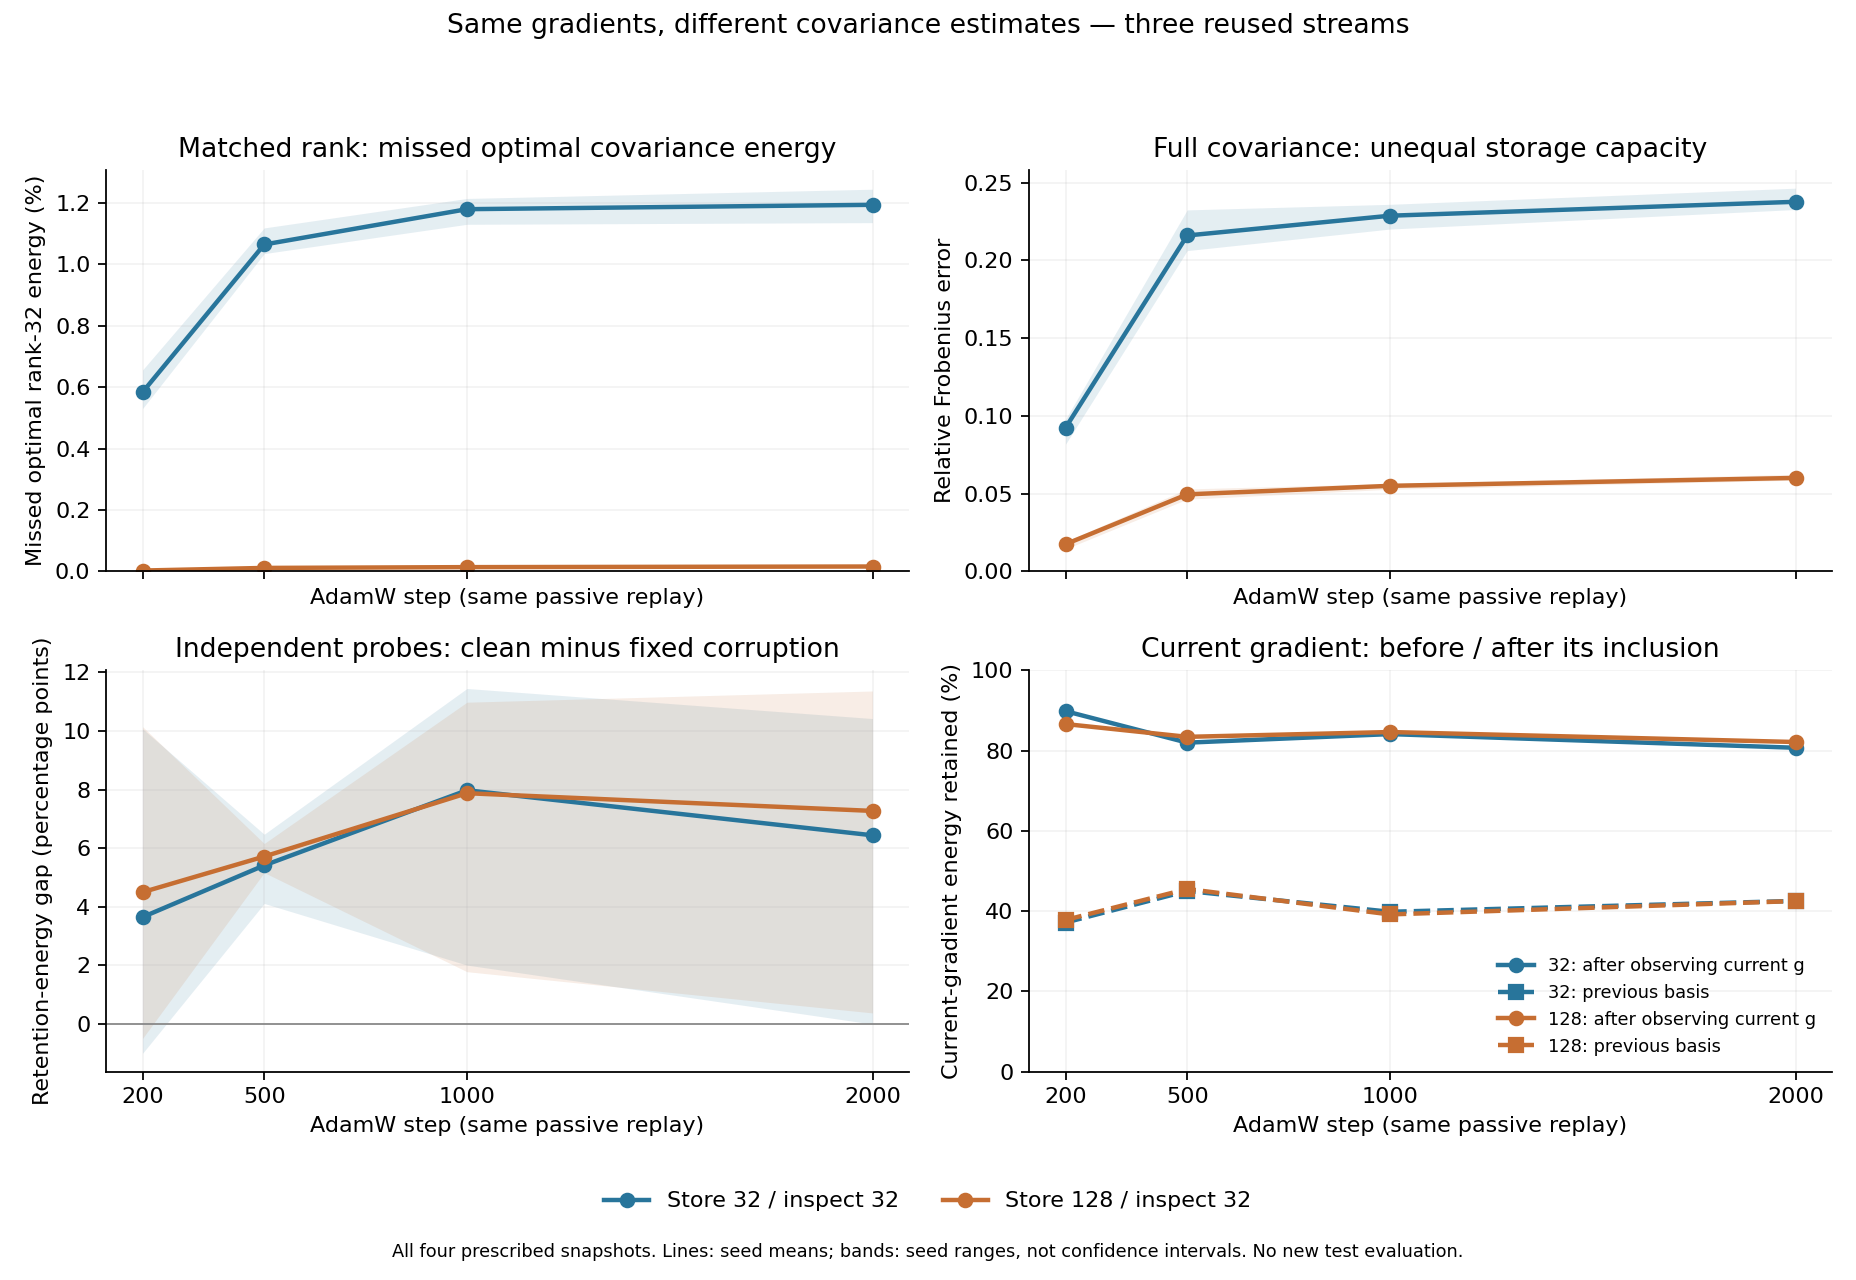
\includegraphics[width=0.95\linewidth,height=\textheight,keepaspectratio,alt={ covariance fidelity, retention and  diagnostics from iteration 005. All four prescribed states are shown; bands are three-seed ranges, not confidence intervals. The  panel shows means only. The upper-left deficit is relative to the rank-32 optimum, not total covariance energy.}]{../continuation/iteration-005/common-stream-diagnostics-v2.png}
\caption{Common-\allowbreak{}stream covariance fidelity, retention and
self-\allowbreak{}inclusion diagnostics from iteration 005. All four
prescribed states are shown; bands are three-seed ranges, not confidence
intervals. The lower-\allowbreak{}right panel shows means only. The
upper-left deficit is relative to the rank-32 optimum, not total
covariance energy.}
\end{figure}

\subsection{5. Mathematical
synthesis}\label{synthesis--mathematical-synthesis}

The \hyperref[mathematics]{mathematical mechanisms report} and
\hyperref[label-noise]{label-\allowbreak{}noise follow-up} provide the
detailed derivations,\allowbreak{} primary-\allowbreak{}source
connections and prior reviews; both accompany this synthesis in the
current PDF edition.

\subsubsection{5.1 What creates the
covariance}\label{synthesis--what-creates-the-covariance}

Condition on current parameters,\allowbreak{} fixed training labels,
past batches and the observer state. Write \(g_t=\bar g_t+\xi_t\), where
\(\bar g_t\) is the conditional batch-\allowbreak{}gradient mean,
\(\operatorname{Cov}(\xi_t)=\Sigma_t\), and \(d_t=\bar g_t-m_{t-1}\).
Then

\[
\mathbb E[c_tc_t^T\mid\mathcal F]
=\beta^2(d_td_t^T+\Sigma_t).
\]

Thus new covariance mass combines \textbf{mean surprise} \(d_td_t^T\)
and fresh conditional batch variability Σ. Mean surprise can reflect
objective drift, representation change, curvature-\allowbreak{}driven
motion, regime change, or noise retained by the lagging mean. It is not
pure clean signal. Fresh variability can itself be
structured.\allowbreak{} The identity describes an ideal
regular-\allowbreak{}weight proposal before native startup, rejection,
pruning, repair, rounding and truncation,\allowbreak{} and expectation
does not commute with eigenvector selection.

At one fixed state, let \(m=m_{t-1}\) be the fixed
pre-\allowbreak{}observation observer mean and \(d=\bar g-m\). Draw
\(g,g'\) conditionally independently from the same
fixed-\allowbreak{}training-\allowbreak{}objective batch
distribution\allowbreak{}.\allowbreak{} Then

\[
\mathbb E[(g-g')(g-g')^T/2\mid\mathcal F]=\Sigma,
\qquad
\mathbb E[(g-m)(g'-m)^T\mid\mathcal F]=dd^T.
\]

Projected scalar versions of these quantities can identify whether
retained activity is dominated by fresh variability or mean surprise
without forming a dense covariance.\allowbreak{} They still do not label
either component useful.

\subsubsection{5.2 PCA solves the wrong objective for general
denoising}\label{synthesis--pca-solves-the-wrong-objective-for-general-denoising}

At a fixed state, let the clean objective gradient be μ and the
corrupted training gradient \(g=\mu+b+\xi\), with
fixed-\allowbreak{}label bias \(b\) and zero-mean fresh noise ξ of
covariance Σ. For an orthogonal projector chosen before that fresh draw,
with the state and target fixed,

\[
R(P)=\mathbb E\|Pg-\mu\|^2
=\|\mu\|^2+\operatorname{tr}\!\left[P(bb^T+\Sigma-\mu\mu^T)\right].
\]

The rank-\(r\) oracle for this MSE retains leading eigenvectors of
\(\mu\mu^T-bb^T-\Sigma\), not leading covariance
eigenvectors\allowbreak{}.\allowbreak{} With varying useful signal
second moment \(M_s\) and independent zero-mean additive noise, the
analogous oracle sees \(M_s-\Sigma\), whereas uncentered PCA sees
\(M_s+\Sigma\). For example, useful variance
\(\operatorname{diag}(4,0)\) and nuisance variance
\(\operatorname{diag}(0,9)\) make rank-one PCA select pure nuisance.
Leading variance is not a usefulness score.

A favorable special case exists: desired gradients lie in a
low-\allowbreak{}dimensional subspace, nuisance is independent and
isotropic, desired coefficients vary enough to appear after centering,
and estimation is independent enough not to overfit the same draw. Under
those assumptions population PCA can recover the desired space. The
current optimizer only approximates them. A constant useful mean may
disappear from centered innovations,\allowbreak{} whereas a
sign-\allowbreak{}alternating nuisance direction can have large
covariance.\allowbreak{}

Even better gradient MSE does not guarantee a better immediate loss
step. For plain SGD with an unbiased gradient and unchanged learning
rate, projection cannot improve the first-\allowbreak{}order
clean-\allowbreak{}descent term beyond the full clean gradient. A
benefit can instead come from reducing curvature cost, suppressing
bias-\allowbreak{}driven fitting, changing finite-\allowbreak{}step
stability, or altering future feature learning. These mechanisms require
distinct measurements\allowbreak{}.\allowbreak{}

\subsubsection{\texorpdfstring{5.3 A fixed-\allowbreak{}Jacobian view:
restriction of learnable
functions}{5.3 A  view: restriction of learnable functions}}\label{synthesis--a-fixed-jacobian-view-restriction-of-learnable-functions}

For square loss with residual \(r=f-y\), fixed Jacobian \(J\), and
\(g=J^Tr/n\), projected SGD gives

\[
\Delta f=-\eta JPJ^Tr/n.
\]

The local kernel becomes \(K_P=JPJ^T\), with
\(0\preceq K_P\preceq JJ^T\). In a linear model this is exact; in a
nonlinear network it is first-\allowbreak{}order and local. The
projector changes which residual components are easy or impossible to
fit through that step. This provides a cohesive explanation for both
noisy-\allowbreak{}label preservation and clean underfitting: the same
restriction helps when wrong-\allowbreak{}label fitting depends on
excluded directions and hurts when useful features do.

It is not a proof that PCA finds the right function modes. If
\(J=USV^T\), then \(C_g=VS(U^TC_rU)SV^T/n^2\); residual covariance and
Jacobian geometry jointly determine the parameter-\allowbreak{}space
spectrum. Nor is \(K_P\) an AdamW kernel. Adding a fixed diagonal
preconditioner produces \(JDPJ^T\), generally nonsymmetric; actual Adam
has historical and input-\allowbreak{}dependent state.

\subsubsection{\texorpdfstring{5.4 Adam limits
gradient-\allowbreak{}space
interpretations}{5.4 Adam limits  interpretations}}\label{synthesis--adam-limits-gradient-space-interpretations}

At a common pre-step Adam state, absorb bias correction into constants
and write the data displacement coordinatewise as

\[
u_i(h)=-\eta\frac{A_i+B h_i}{\sqrt{C_i+D h_i^2}+\epsilon}.
\]

Changing \(h\) changes numerator and denominator.\allowbreak{} On the
first step with zero moments and negligible ε, the displacement is
approximately \(-\eta\operatorname{sign}(h_i)\), so input magnitude can
largely disappear. Later, old momentum can move parameters even under
zero current gradient; diagonal scaling can rotate a vector out of a
non-\allowbreak{}coordinate subspace; and decay contributes
independentl\allowbreak{}y.\allowbreak{} I2 supplies an exact existence
example, while I3 shows that corresponding
leakage-\allowbreak{}associated direction reversals are rare in the
measured noisy-\allowbreak{}MNIST trajectory.\allowbreak{} Mathematical
possibility and empirical frequency are separate
conclusions.\allowbreak{}

I4 and I6 show why norm language must be precise. Scaling the raw
gradient to the norm of its hypothetical projection does not match the
filtered arm's Adam moments or step. Restoring the lagged
projected-\allowbreak{}gradient norm does not restore the current arm's
step. Conversely,\allowbreak{} I6 clean filtering has larger mean
data-step norm than AdamW while learning less. Neither ``smaller steps''
nor ``direction alone'' is identified.\allowbreak{} The base optimizer
is part of the intervention\allowbreak{}.\allowbreak{}

\subsubsection{\texorpdfstring{5.5 Fixed corruption,\allowbreak{} fresh
labels, and the retention
ceiling}{5.5 Fixed  fresh labels, and the retention ceiling}}\label{synthesis--fixed-corruption-fresh-labels-and-the-retention-ceiling}

For logits \(z\), probabilities \(p\), parameter Jacobian \(J\), clean
target \(y\), and a fresh uniform-\allowbreak{}replacement label
\(\tilde y\) at rate ρ,

\[
g_y=J^T(p-e_y),\quad
q=(1-\rho)e_y+\rho\mathbf1/K,\quad
g_{\tilde y}=g_q+\varepsilon_{\tilde y},
\]

where \(g_q=J^T(p-q)\) and
\(\mathbb E[\varepsilon_{\tilde y}\mid\theta,x,y]=0\) only for the
indicated fresh independent redraw. The existing trained
fixed-\allowbreak{}corruption residual does not inherit this conditional
identity. Old labels helped determine θ; drawing new minibatch indices
does not make those assignments fresh. The missing
soft-\allowbreak{}target gradient \(g_q\) cannot be reconstructed from
retained clean/\allowbreak{}residual aggregates and requires a new probe
acquisition.\allowbreak{}

Fresh label randomness is structured after the Jacobian:

\[
\operatorname{Cov}(g_{\tilde y}\mid\theta,x,y)
=J^T[\operatorname{diag}(q)-qq^T]J.
\]

For \(K=10,\rho=.9\), the nonzero label-\allowbreak{}space eigenvalues
are .09 on the eight wrong-\allowbreak{}class contrast directions and
.171 on the true-\allowbreak{}versus-\allowbreak{}others direction. At
\(p=q\) and with locally twice-\allowbreak{}differentiab\allowbreak{}le
logits, this covariance equals the per-input expected
cross-\allowbreak{}entropy Hessian: the residual-\allowbreak{}weighted
logit-\allowbreak{}Hessian term vanishes. This is not a claim about the
observed temporal covariance.\allowbreak{} Thus a covariance direction
can look curvature-\allowbreak{}like precisely because of random labels;
curvature alignment alone is not evidence of clean semantic signal.

At uniform predictions,\allowbreak{} the expected fresh corruption
residual is exactly \(-\rho g_y\). Any fixed homogeneous linear filter
retains the same normalized energy of these antiparallel mean vectors.
This illustrates a sign-\allowbreak{}blindness limit, not an assertion
that I5 predictions were uniform or its realized residuals equal their
fresh-\allowbreak{}label means.

The strong clean/\allowbreak{}residual opposition in I5 also has a
precise limit. For nonzero vectors \(c,r\), cosine γ, and any ideal
nontrivial orthoprojector \(P\),

\[
\left|
\frac{\|Pc\|^2}{\|c\|^2}-
\frac{\|Pr\|^2}{\|r\|^2}
\right|\le\sqrt{1-\gamma^2}.
\]

Across all twelve retained I5 states, mean cosine is −.881220 and the
mean ideal absolute-\allowbreak{}gap ceiling is .469728. Observed signed
clean-\allowbreak{}minus-\allowbreak{}residual gaps are only .058674 for
width32 and .063387 for width128. At final states, the corresponding
values are cosine −.896945, ceiling .441290, and gaps .064382/ .072703.
Opposition limits possible selectivity but leaves substantial ideal
headroom; it does not force the observed gaps to be small. The ceiling
is an oracle geometric maximum, not a native guarantee or promised
performance gain. The maximizing projector need not be learnable,
stable, or good for training. See the complete
\hyperref[label-noise]{identifiability analysis}.

\subsection{6. Ranked hypotheses and falsifiable
tests}\label{synthesis--ranked-hypotheses-and-falsifiable-tests}

The hypotheses overlap; the ranking expresses current explanatory value,
not posterior probabilitie\allowbreak{}s.\allowbreak{} Confidence
concerns the existing evidence, not a claim that one mechanism acts
alone.

\subsubsection{1. Learned directional regularization --- moderate
confidence}\label{synthesis--learned-directional-regularization-moderate-confidence}

The filter changes which gradient information enters AdamW, suppresses
late wrong-\allowbreak{}label fitting in multiple selected recipes, and
does something the tested scalar attenuation controls do not reproduce.
It also underfits clean MNIST and CIFAR, delays parity, and fails to
transfer uniformly. This broad account fits both benefits and costs
without assuming semantic eigendirecti\allowbreak{}ons.\allowbreak{}

\textbf{Potential contradiction:} accuracy-\allowbreak{}selected effects
against AdamW reverse between I4 and I6, and clean/\allowbreak{}residual
retention selectivity is small and
heterogeneou\allowbreak{}s.\allowbreak{} A learned orientation could be
epiphenomenal while effective capacity, history, or
optimizer-\allowbreak{}state changes cause the outcome.

\textbf{Falsifiable test:} at identical complete states, compare
filtered and raw data displacements after artificially matching
\emph{actual displacement norm}, then add identical decay. Evaluate
finite loss changes on independent clean,
fixed-\allowbreak{}corruption,\allowbreak{} fresh-\allowbreak{}redraw
and soft-\allowbreak{}target probes. If learned orientation does not
improve any predeclared
clean-\allowbreak{}versus-\allowbreak{}corruption utility contrast, or
if random orientations with matched displacement perform equivalently
within prespecified precision, that local directional account weakens. A
null one-step effect would not exclude a mechanism operating through
later states.

\subsubsection{2. Adam history and adaptive scaling mediate the effect
--- interaction certain, causal contribution
unresolved}\label{synthesis--adam-history-and-adaptive-scaling-mediate-the-effect-interaction-certain-causal-contribution-unresolved}

Noncommutation and moment carryover are mathematical facts; neural
trajectories show large out-\allowbreak{}of-\allowbreak{}subspace step
energy and failures of input-norm matching to match steps. What remains
unknown is how much this interaction causes the long-run
anti-\allowbreak{}memorization\allowbreak{} rather than merely
accompanying it.

\textbf{Potential contradiction:} the filter changes learning even
though Adam often leaves its nominal subspace, which could mean the
important effect occurs in the moments' information content rather than
geometric confinement.\allowbreak{} Rare observed ascent reversal argues
against using the I2 pathology as a generic explanation.\allowbreak{}

\textbf{Falsifiable test:} clone parameters,\allowbreak{} buffers,
observer, Adam moments, counters, scheduler and RNG at the same state.
Feed raw, current-\allowbreak{}basis,\allowbreak{}
previous-\allowbreak{}basis and zero gradients on the same batch. Record
data-only and total displacement\allowbreak{}s,\allowbreak{} projected
leakage, logits and independent probe losses. Repeat with separately
specified SGD or reprojected-\allowbreak{}Adam displacement controls. A
small, stable difference between gradient-\allowbreak{}space predictions
and realized utility would weaken the chosen immediate-\allowbreak{}step
mediation prediction; a sign-\allowbreak{}changing difference would
support it. Neither alone bounds Adam's long-run causal role.

\subsubsection{\texorpdfstring{3. Covariance primarily tracks a mixture
of mean drift, curvature-\allowbreak{}driven motion, and batch
variability --- moderate mathematical\allowbreak{},\allowbreak{} low
neural
confidence}{3. Covariance primarily tracks a mixture of mean drift,  motion, and batch variability --- moderate  low neural confidence}}\label{synthesis--covariance-primarily-tracks-a-mixture-of-mean-drift-curvature-driven-motion-and-batch-variability-moderate-mathematical-low-neural-confidence}

The conditional identity includes mean surprise and fresh
variability,\allowbreak{} and the centered filter emphasizes temporal
change. A scalar quadratic shows that equal injected noise can create
different gradient variance as curvature and learning-\allowbreak{}rate
dynamics approach oscillation.\allowbreak{} Structured label covariance
can itself resemble curvature.

\textbf{Potential contradiction:} these sources may explain the spectrum
while remaining irrelevant to which information affects
generalizati\allowbreak{}on.\allowbreak{}

\textbf{Falsifiable test:} at frozen states, use independent batch pairs
to estimate fresh-\allowbreak{}variability and
mean-\allowbreak{}surprise energy along retained, discarded and random
comparison directions.\allowbreak{} Only if mean surprise dominates
should a second stage measure gradient temporal autocorrelation and
Hessian-\allowbreak{}vector response. Failure of these quantities to
predict same-state utility would reject them as useful mediators even if
they reconstruct covariance energy.

\subsubsection{\texorpdfstring{4. Recursive truncation causes useful
path-\allowbreak{}dependent learning delay --- high estimator, low
learning
confidence}{4. Recursive truncation causes useful  learning delay --- high estimator, low learning confidence}}\label{synthesis--recursive-truncation-causes-useful-path-dependent-learning-delay-high-estimator-low-learning-confidence}

I1 establishes the delay on controlled streams, and I5 shows wider
storage is more faithful to the chosen finite-\allowbreak{}history
reference. But exact or wider covariance is not an oracle, width can be
nonmonotone in analytical examples, and filtered trajectories show
adverse width seeds.

\textbf{Falsifiable test:} use common saved gradient streams and
complete states to compare narrow, wide and exact-\allowbreak{}reference
leading spaces on independent one-step utility. Predeclare
turnover/\allowbreak{}admission metrics. If improved capture predicts
neither useful-\allowbreak{}gradient action nor cleaner
displacement\allowbreak{},\allowbreak{} estimator fidelity is not the
operative learning mechanism. A later whole-\allowbreak{}policy
comparison is warranted only after this bridge is positive.

\subsubsection{\texorpdfstring{5. Self-\allowbreak{}inclusion is mainly
a tracking mechanism, not useful denoising ---
low-\allowbreak{}to-\allowbreak{}moderate
confidence}{5.  is mainly a tracking mechanism, not useful denoising ---  confidence}}\label{synthesis--self-inclusion-is-mainly-a-tracking-mechanism-not-useful-denoising-low-to-moderate-confidence}

I5 measures a very large current-\allowbreak{}versus-\allowbreak{}prior
retention change, but I6 finds no dependable benefit from lagging. This
favors the view that self-\allowbreak{}inclusion helps the basis follow
the current regime, though its utility varies.

\textbf{Potential contradiction:} I6 is small and
whole-\allowbreak{}policy; on noisy data its sign reverses across
bundles. Lagging changes direction, magnitude, moments and future states
together.

\textbf{Falsifiable test:} in complete-\allowbreak{}state one-step
clones, compare current and prior bases with reciprocal displacement
matching and independent probes. Test whether the
self-\allowbreak{}included component disproportionately benefits
training-\allowbreak{}batch loss while harming independent
objectives.\allowbreak{} Do not treat current-\allowbreak{}gradient
retention as independent evidence.

\subsubsection{\texorpdfstring{6. Ordinary training restraint explains
most endpoint gains --- plausible alternative,\allowbreak{} currently
weakened but not ruled
out}{6. Ordinary training restraint explains most endpoint gains --- plausible  currently weakened but not ruled out}}\label{synthesis--ordinary-training-restraint-explains-most-endpoint-gains-plausible-alternative-currently-weakened-but-not-ruled-out}

The collapse from endpoint to accuracy-\allowbreak{}selected advantage
makes early stopping an important alternative.\allowbreak{} The I4
scalar control fails to reproduce endpoints, so one
own-\allowbreak{}trajectory gradient-\allowbreak{}norm policy is
insufficient\allowbreak{}.\allowbreak{} That does not cover
validation-\allowbreak{}tuned stopping, learning-\allowbreak{}rate
schedules, weight decay, update-\allowbreak{}norm controls or reduced
capacity.

\textbf{Falsifiable test:} predeclare a fair tuning budget and compare
spectral training with validation-\allowbreak{}accuracy and
validation-\allowbreak{}CE early stopping,
warmup-\allowbreak{}stop,\allowbreak{}
learning-\allowbreak{}rate/\allowbreak{}weight-\allowbreak{}decay
baselines, reduced-\allowbreak{}width models, and
actual-\allowbreak{}step-\allowbreak{} matched controls. Keep an
untouched final test and report endpoint and selected estimands
separately.\allowbreak{} If simpler restraint matches the Pareto
frontier, the spectral geometry has limited incremental value.

\subsubsection{Prioritized
resources}\label{synthesis--prioritized-resources}

The first two diagnostic families fit the existing small MLP scale and
can be CPU/GPU bounded after a short pilot; they require
complete-\allowbreak{}state acquisition because old model-only
checkpoints cannot reconstruct exact Adam and observer
counterfactu\allowbreak{}als.\allowbreak{} A
three-\allowbreak{}to-\allowbreak{}five-\allowbreak{}paired-\allowbreak{}seed
whole-\allowbreak{}policy follow-up could run on the local RTX 3090 or
free MATS L40 partition only after those diagnostics and a frozen
analysis plan. CIFAR attack replay, fresh purged Numerai folds, and 7B
language-\allowbreak{}model training or rejudging are later and require
separate runtime, cost and metric approval. No paid compute is implied
here.

\subsection{7. Limitations and their
disposition}\label{synthesis--limitations-and-their-disposition}

{\def\LTcaptype{none} % do not increment counter
\begin{longtable}[]{@{}
  >{\raggedright\arraybackslash}p{(\linewidth - 4\tabcolsep) * \real{0.3333}}
  >{\raggedright\arraybackslash}p{(\linewidth - 4\tabcolsep) * \real{0.3333}}
  >{\raggedright\arraybackslash}p{(\linewidth - 4\tabcolsep) * \real{0.3333}}@{}}
\toprule\noalign{}
\begin{minipage}[b]{\linewidth}\raggedright
Limitation
\end{minipage} & \begin{minipage}[b]{\linewidth}\raggedright
Current disposition
\end{minipage} & \begin{minipage}[b]{\linewidth}\raggedright
What would resolve it
\end{minipage} \\
\midrule\noalign{}
\endhead
\bottomrule\noalign{}
\endlastfoot
Ambiguous algorithm identity & \textbf{Resolved for the canonical code:}
temporal centered covariance,\allowbreak{} sample-\allowbreak{}space
consensus, matrix-\allowbreak{}gradient spectra and adapter spectra are
separated. & Keep implementation labels and hashes in every future
claim. \\
Numerical stability versus statistical approximation & \textbf{Resolved
conceptually:} the stable update repairs geometry but recursive
truncation remains approximate.\allowbreak{} I1/I5 support the
distinction.\allowbreak{} & Common-\allowbreak{}state utility tests
determine whether fidelity matters
scientifical\allowbreak{}ly.\allowbreak{} \\
Endpoint versus stopping-\allowbreak{}policy claims &
\textbf{Acknowledged and directly measured:} I4 shows +18.81 endpoint
but −2.38 accuracy-\allowbreak{}selected points; I6's selected sign
reverses. & Fresh, preregistered tuning and untouched-\allowbreak{}test
comparisons.\allowbreak{} \\
``Gradient denoising'' semantics & \textbf{Not established:} covariance
magnitude, gradient MSE, loss descent and generalization are different
objectives.\allowbreak{} &
Clean/\allowbreak{}soft-\allowbreak{}target/\allowbreak{}fixed-\allowbreak{}residual
probes and displacement\allowbreak{}-\allowbreak{}matched causal
tests. \\
Fixed-\allowbreak{}corruption residual treated as fresh zero-mean noise
& \textbf{Corrected:} the conditional identity applies to fresh redraws,
not old trained assignments.\allowbreak{} & Acquire the missing
soft-\allowbreak{}target gradient and fresh-\allowbreak{}redraw probes
under new scope. \\
Strong clean/\allowbreak{}residual opposition & \textbf{Quantified:} it
limits selectivity but does not explain the small observed gaps; large
ideal headroom remains. & Native/\allowbreak{}common-\allowbreak{}state
comparisons may test attainable rather than oracle
selectivity.\allowbreak{} \\
Pre-Adam projection interpreted as subspace training & \textbf{Resolved
as false in general; measured leakage is large.} Its causal importance
remains open. & Complete-\allowbreak{}state
Adam/\allowbreak{}SGD/\allowbreak{}reprojected-\allowbreak{}step
comparisons.\allowbreak{} \\
Norm controls & \textbf{Narrowly resolved:} I4 scalar attenuation and I6
projection-\allowbreak{}norm restoration do not reproduce all outcomes.
Neither matches actual steps. & Direct reciprocal displacement
matching. \\
Wider estimation & \textbf{Established as more faithful on tested common
streams, not universally better or causally useful.} & Link fidelity to
independent utility before another policy study. \\
Self-\allowbreak{}inclusion & \textbf{Measured as large; benefit
unresolved.\allowbreak{}} I6 rules out a consistent lagging benefit in
its scope. & Same-state current/\allowbreak{}prior intervention with
matched displacement and more independent bundles if justified. \\
Adversarial robustness & \textbf{Negative boundary condition with
audited stored arrays; attacks not independently replayed.} & Fresh
retained adversarial examples, matched layouts/\allowbreak{}horizons and
certified or stronger attacks. \\
Numerai transfer & \textbf{Candidate failure observed; optimizer
causality confounded and Diagnostics raw export missing.} & Fixed
architecture\allowbreak{}/\allowbreak{}exposure on purged temporal folds
or recovery of the historical export. \\
EM scoring & \textbf{Input-\allowbreak{}processing defect verified;
corrected effect unknown.} & Frozen, consistently stripped,
all-\allowbreak{}response rescoring with repeated seeds and proper
controls. \\
Generality & \textbf{Unresolved:} most clean mechanism evidence uses one
small MNIST MLP and few bundles. & Transfer only after same-state
mechanism predictions are preregistere\allowbreak{}d.\allowbreak{} \\
\end{longtable}
}

Several apparently reassuring quantities must not be overread. The I5
ideal rank-32 reference is a covariance approximation target, not
semantic truth. The label-\allowbreak{}retention ceiling is an oracle
upper bound, not a native guarantee or performance headroom. An ideal
recurrence with regular observation weighting is not the exact native
algorithm at startup or under rejection, repair, truncation and floating
point. Numerical audits validate recorded computations; they do not turn
three seeds into population inference.

\subsection{8. Related primary
work}\label{synthesis--related-primary-work}

The closest literature clarifies concepts; none validates this optimizer
by analogy.

\begin{itemize}
\tightlist
\item
  \href{https://arxiv.org/abs/1812.04754}{Gur-Ari, Roberts and Dyer}
  report gradient concentration in small Hessian-\allowbreak{}related
  subspaces. Their result motivates low-\allowbreak{}dimensional
  tracking but does not make centered temporal covariance a
  useful-\allowbreak{}gradient oracle.
\item
  \href{https://arxiv.org/abs/2405.16002}{Song, Ahn and Yun} show that
  projecting onto dominant Hessian directions can stall learning while
  removing them can preserve progress. High energy and productive
  descent are not equivalent.\allowbreak{}
\item
  \href{https://arxiv.org/abs/1806.07572}{Jacot, Gabriel and Hongler}
  provide the neural-\allowbreak{}tangent-\allowbreak{}kernel framework
  used for the fixed-\allowbreak{}Jacobian analogy. The present finite
  ReLU/AdamW trajectories are not a frozen-\allowbreak{}kernel theorem.
\item
  \href{https://arxiv.org/abs/1706.05394}{Arpit et al.} document early
  pattern learning and later memorization of random labels, making
  selective slowing a plausible outcome. They do not identify this
  filter's mechanism.
\item
  \href{https://arxiv.org/abs/1905.12558}{Kunstner, Balles and Hennig}
  explain why empirical gradient second moments should not casually be
  called Fisher or Hessian matrices. The warning is stronger for
  centered temporal covariance.\allowbreak{}
\item
  \href{https://arxiv.org/abs/1501.01711}{Ghashami et al.} give Frequent
  Directions sketch guarantees,\allowbreak{} helping separate covariance
  approximation from downstream utility. Those guarantees do not apply
  to this recursively truncated EMA.
\item
  \href{https://arxiv.org/abs/2403.03507}{GaLore},
  \href{https://proceedings.mlr.press/v80/gupta18a.html}{Shampoo}, and
  \href{https://arxiv.org/abs/2409.11321}{SOAP} show why matrix layout
  and optimizer- state placement must be specified. Their spectral
  objects and interventions differ from temporal global filtering.
\item
  \href{https://arxiv.org/abs/1705.08292}{Wilson et al.} support
  treating adaptive optimization as part of the inductive bias.
\item
  \href{https://arxiv.org/abs/1906.05271}{Feldman} shows why
  memorization of rare examples can support
  generalizati\allowbreak{}on.\allowbreak{} Suppressing memorization is
  not intrinsically beneficial.\allowbreak{}
\item
  \href{https://arxiv.org/pdf/1512.00567}{Szegedy et al.} introduce the
  soft-\allowbreak{}target view used in label smoothing;
  \href{https://papers.neurips.cc/paper_files/paper/2019/hash/f1748d6b0fd9d439f71450117eba2725-Abstract.html}{Müller,
  Kornblith and Hinton} and
  \href{https://arxiv.org/abs/2003.02819}{Lukasik et al.} study its
  calibration,\allowbreak{} representation and noisy-\allowbreak{}label
  effects. None shows that the spectral filter implements label
  smoothing.
\end{itemize}

``Spectral bias'' in Fourier function learning,
sample-\allowbreak{}gradient agreement, low-rank
optimizer-\allowbreak{}state compression and adapter singular spectra
are useful neighboring ideas but not interchangeable claims. This
investigation makes no publication-\allowbreak{}standard novelty or
state-\allowbreak{}of-\allowbreak{}the-\allowbreak{}art claim.

\subsection{9. Conclusion and current
status}\label{synthesis--conclusion-and-current-status}

The evidence supports one robust practical statement: selected temporal
hard filters can strongly suppress late memorization of randomly
corrupted training labels. It does not support the broader statement
that dominant temporal gradient-\allowbreak{}covariance directions are
generally clean, useful, robust, aligned or economically
persistent.\allowbreak{} Noise can be structured; useful means can
vanish under centering; recursive memory can delay new features; and
Adam can transform a projected gradient into a step outside the nominal
space.

The current synthesis is therefore conditional.\allowbreak{} The
optimizer most likely acts as learned directional
regularizati\allowbreak{}on,\allowbreak{} altering which local function
changes remain learnable, with Adam history and adaptive scaling
mediating the real intervention\allowbreak{}.\allowbreak{} This account
accommodates endpoint
anti-\allowbreak{}memorization\allowbreak{},\allowbreak{} clean
underfitting\allowbreak{},\allowbreak{} opposing grokking results,
negative robustness,\allowbreak{} unstable
selected-\allowbreak{}checkpoint gains, and
application-\allowbreak{}transfer failures. It remains a provisional
mechanism because no same-\allowbreak{}complete-\allowbreak{}state
causal measurement yet connects learned covariance directions to
independent clean-\allowbreak{}versus-\allowbreak{}corruption utility
after actual displacement is controlled.\allowbreak{}

The next decisive question is not ``does PCA keep the good gradient?''
but: \textbf{which task-\allowbreak{}relevant function changes become
easier or harder after the history-\allowbreak{}dependent filter and
AdamW interact, and can those changes be predicted from measurements
made before the outcome?} Complete-\allowbreak{}state one-step
comparisons and independent-\allowbreak{}batch
covariance-\allowbreak{}source probes are the shortest path to an
answer. Only a positive predictive bridge would justify a further
whole-\allowbreak{}policy or expensive application study.

As of 7 September 2026, no experiment is running. Iteration 007
preparation made no native training run and produced no new scientific
evidence: its fixed one-shot service has MainPID 0, exited with status
2, and left an invalid zero-byte measurement file. The failure is
preserved and consumed; any repaired replacement requires explicit
authorization and a new scope. This report does not announce a launch,
permission,\allowbreak{} retry, default change, or completion of the
broader continuing investigatio\allowbreak{}n.\allowbreak{}

\clearpage

\section{Appendix A. Mathematical mechanisms and ranked
hypotheses}\label{mathematics}

Codex / Spectral Optimizer Investigation --- mathematical synthesis, 7
September 2026.

\subsection{High-level
assessment}\label{mathematics--high-level-assessment}

My leading hypothesis is \textbf{task-\allowbreak{}dependent directional
regularizati\allowbreak{}on,\allowbreak{} strongly mediated by Adam},
not a general-\allowbreak{}purpose separation of signal from noise. The
filter changes which gradient information reaches the optimizer. Under
some noisy-\allowbreak{}label recipes, that appears to restrict late
memorization while retaining useful early learning. The same restriction
can obstruct useful learning on clean data or other tasks. Which changes
survive Adam's historical moments and coordinatewise scaling remains a
central unanswered question.

Confidence is high in the mathematical distinctions below, moderate in
this broad interpretation of the empirical pattern, and low in any
uniquely identified causal mechanism. The stronger claim that leading
covariance directions are intrinsically useful is false in general.
Better covariance estimation,\allowbreak{} better gradient
estimation,\allowbreak{} better immediate loss, and better eventual
generalization are four different
achievements\allowbreak{}.\allowbreak{}

This addendum supplies additional reasoning and proposed tests, not new
training results. No experiment is currently running: the one-shot I7
storage check failed without a retained candidate and is preserved. Its
\href{../continuation/iteration-007/native-storage-measurement-failure-review.md}{failure
record} does not change the scientific evidence. The original report/PDF
and optimizer implementation remain unchanged.

\subsection{1. What the actual code
measures}\label{mathematics--what-the-actual-code-measures}

The canonical hard filter observes the flattened \textbf{raw batch-mean
gradient}, updates its running mean, estimates a low-rank covariance of
the centered innovation,\allowbreak{} then projects the same raw
gradient before AdamW sees it:

\[
a_t=\beta a_{t-1}+(1-\beta)g_t,\qquad
c_t=g_t-a_t=\beta(g_t-a_{t-1}),\qquad h_t=P_tg_t.
\]

Here \(P_t\) denotes the ideal orthogonal projector. Actual stored
columns give the finite-\allowbreak{}precision action \(V_t(V_t^Tg_t)\).
The first gradient initializes the mean; the first nonzero innovation
initializes covariance without the later \(1-\beta\) weight; subsequent
updates truncate repeatedly.\allowbreak{} These differ from PCA on an
exact, independently sampled covariance.\allowbreak{} See
\href{../../../spectral_filter.py}{the code} and the prior
\href{../analysis/mathematical-audit.md}{implementation audit}.

A useful new decomposition conditions on the current
parameters,\allowbreak{} fixed training labels, past batches and
observer state. Write \(g_t=\bar g_t+\xi_t\), with conditional mean
\(\bar g_t\), noise covariance \(\Sigma_t\), and
\(d_t=\bar g_t-a_{t-1}\). Then

\[
\mathbb E[c_tc_t^T\mid\mathcal F]=\beta^2(d_td_t^T+\Sigma_t).
\]

An ideal regular-\allowbreak{}weight,\allowbreak{}
complete-\allowbreak{}innovation covariance proposal therefore has
expectation \(\beta C_{t-1}+(1-\beta)\beta^2(d_td_t^T+\Sigma_t)\). New
covariance mass mixes \textbf{mean surprise} and \textbf{fresh batch
variability}. Mean surprise includes both changes in the objective
gradient and noise remembered by the lagging mean; it is not pure
curvature or pure signal. This describes the ideal proposal, not the
native result after residual rejection, pruning, repair, rounding,
startup exceptions or rank truncation.\allowbreak{} Expectation does not
commute with selecting eigenvectors\allowbreak{}.\allowbreak{}

This leads to a cheap proposed diagnostic.\allowbreak{} At one unchanged
state, two independent batches satisfy

\[
\mathbb E[(g-g')(g-g')^T/2\mid\mathcal F]=\Sigma,\qquad
\mathbb E[(g-a)(g'-a)^T\mid\mathcal F]=dd^T.
\]

We can estimate these \textbf{along selected directions}, without a
dense covariance.\allowbreak{} That distinguishes why a direction has
high activity before asking whether it is useful. See the
\href{../analysis/mathematical-followup-covariance.md}{covariance
derivation}.

\subsection{2. Covariance magnitude is not a usefulness
score}\label{mathematics--covariance-magnitude-is-not-a-usefulness-score}

At a fixed state, let \(\mu\) be a clean-\allowbreak{}objective gradient
and write the corrupted-\allowbreak{}training gradient as
\(g=\mu+b+\xi\). Fixed-\allowbreak{}label bias \(b\) need not vanish.
For a projector chosen before the fresh batch,

\[
R(P)=\mathbb E\|Pg-\mu\|^2
=\|\mu\|^2+\operatorname{tr}[P(bb^T+\Sigma-\mu\mu^T)].
\]

An oracle restricted to rank-\(r\) orthogonal projectors minimizes this
risk with the leading eigenspace of \(\mu\mu^T-bb^T-\Sigma\),
\textbf{not gradient covariance}. This compares mathematical
objectives,\allowbreak{} not deployable rules: the clean target and
nuisance statistics are unknown, and a single-\allowbreak{}state target
does not describe a changing gradient field.

For a varying useful signal with second moment \(M_s\) and independent
noise, the analogous risk selects \(M_s-\Sigma\), whereas uncentered PCA
sees \(M_s+\Sigma\). Useful variance \(\operatorname{diag}(4,0)\) and
noise variance \(\operatorname{diag}(0,9)\), for example, make rank-one
PCA keep pure noise. This is an analytical
counterexamp\allowbreak{}le,\allowbreak{} not a newly sampled
experiment.\allowbreak{}

A favorable special case is useful mean and variation confined to a
subspace, isotropic independent noise, and nonzero signal variation in
every desired direction. Population PCA can identify the subspace, and
an independently evaluated projector removes noise outside it. The
current method must approximate these conditions,\allowbreak{} not
assume them. A constant useful mean may never enter centered
covariance.\allowbreak{}

Reduced gradient MSE still does not establish a better loss step. For
plain SGD, an unbiased gradient and the same learning rate, projection
cannot improve the first-\allowbreak{}order clean-\allowbreak{}descent
term beyond \(\|\mu\|^2\). Benefits can concern
curvature/\allowbreak{}noise costs, biased fitting or future learning
instead. The earlier
\href{../continuation/predictable-projection-theory.md}{predictable-\allowbreak{}projection
analysis} already gives a counterexample where MSE improves while
expected clean loss worsens. Adam requires a different analysis.

\subsection{3. A better bridge: which functions remain easy to
learn?}\label{mathematics--a-better-bridge-which-functions-remain-easy-to-learn}

Consider a fixed-\allowbreak{}Jacobian square-\allowbreak{}loss proxy:
outputs \(f\), residual \(r=f-y\), Jacobian \(J\), and loss
\(\|r\|^2/(2n)\). Then

\[
g=J^Tr/n,\qquad C_g=J^TC_rJ/n^2,\qquad
\Delta f=-\eta JPJ^Tr/n.
\]

The last equality is exact for a linear model and
first-\allowbreak{}order for a nonlinear one. Projected SGD replaces the
tangent kernel \(JJ^T\) by \(K_P=JPJ^T\), with
\(0\preceq K_P\preceq JJ^T\). It restricts local
function-\allowbreak{}space learning. With a fixed kernel,
small-\allowbreak{}eigenvalue residual components learn slowly; removed
directions do not learn through that update.

This offers a coherent hypothesis for both outcomes: restriction helps
if fitting wrong labels needs directions that can be suppressed while
useful structure remains accessible; it hurts if useful learning needs
those same excluded directions.\allowbreak{} It resembles selective
slowing or stopping of modes, not a detector of label truth. Unlike
simply stopping training, filtered policies can continue improving after
warmup; the earlier studies measure that too.

The \href{https://arxiv.org/abs/1806.07572}{neural tangent kernel
connection} is a controlled analogy, not a claim that this finite ReLU
network has a frozen kernel throughout training. PCA does not
automatically choose the top kernel modes: if \(J=USV^T\), then
\(C_g=VS(U^TC_rU)SV^T/n^2\). Residual covariance must have suitable
alignment. Structured noise and changing representations can alter it.

Fixed diagonal preconditioning after projection instead gives
\(JDPJ^T\), generally nonsymmetric and not a PSD kernel. Actual Adam
also has historical moments and an input-\allowbreak{}dependent
denominator.\allowbreak{} The simple kernel story supplies hypotheses
and tests, not an AdamW theorem.

\subsection{4. High activity may come from optimization
dynamics}\label{mathematics--high-activity-may-come-from-optimization-dynamics}

The centering transfer function is \(\beta(1-z^{-1})/(1-\beta z^{-1})\):
it rejects a constant component and responds to change. Covariance then
averages outer-\allowbreak{}product power. It forgets global sign, not
all relative coordinate signs or phases. Alternating gradients can
therefore receive high covariance energy despite zero signed agreement.

A new local calculation makes the curvature connection concrete. In
stationary scalar quadratic SGD, let

\[
g_t=he_t+\xi_t,\quad e_{t+1}=(1-\eta h)e_t-\eta\xi_t,\quad
0<\eta h<2,\quad \operatorname{Var}(\xi_t)=\sigma^2.
\]

Then \(\operatorname{Var}(g_t)=2\sigma^2/(2-\eta h)\). Equal injected
noise can produce different gradient variances as curvature and learning
rate change. Near the oscillatory stability boundary, covariance can be
large because optimization is oscillating.\allowbreak{} Centering does
not remove that high-\allowbreak{}frequency component. This is exact for
the stated toy system, not a measured property of the neural runs. The
\href{../analysis/mathematical-followup-main-derivations.md}{derivation
note} gives the full transfer spectrum.

This motivates directional temporal correlations and, if warranted,
Hessian-\allowbreak{}vector responses after the simpler
fixed-\allowbreak{}state batch-pair
decompositio\allowbreak{}n.\allowbreak{} Calling the covariance a Fisher
matrix, Hessian, or semantic feature covariance would skip the question
we need to answer.

\subsection{5. Why Adam must be part of the
mechanism}\label{mathematics--why-adam-must-be-part-of-the-mechanism}

At the same pre-step Adam state, bias correction can be absorbed into
constants so its data displacement is

\[
u_i(h)=-\eta\frac{A_i+B h_i}{\sqrt{C_i+D h_i^2}+\epsilon}.
\]

Both numerator and denominator change with the delivered gradient. On a
first step with zero moments and negligible epsilon, this is
approximately \(-\eta\operatorname{sign}(h_i)\): changing magnitude need
not change the step. Later, history changes the response. Momentum spans
historical gradient spaces; diagonal scaling can leave even a fixed
rotated subspace; decay adds another
displacement\allowbreak{}.\allowbreak{} Equal gradient norms do not
match update norms, update directions,\allowbreak{} function changes or
future state.

This is not only hypothetical\allowbreak{}.\allowbreak{} In
\href{../continuation/iteration-004/summary.json}{iteration 004}, scalar
gradient attenuation left mean data-step norms close to AdamW's, while
hard filtering produced smaller ones. Yet smaller steps are not a
universal explanation: in
\href{../continuation/iteration-006/results.md}{iteration 006}, clean
filtered training had larger mean data-step norm than AdamW and learned
less. These are different trajectories\allowbreak{},\allowbreak{} so
neither observation alone identifies a mediator. They make
complete-\allowbreak{}state comparisons more informative than another
unmatched norm control.

\subsection{6. Ranked hypotheses against the existing
evidence}\label{mathematics--ranked-hypotheses-against-the-existing-evidence}

These explanations can coexist. The ranking is a research judgment, not
fitted posterior probabilitie\allowbreak{}s.\allowbreak{} Every proposed
falsifier concerns a specified regime and needs adequate precision
around a predeclared meaningful effect size.

{\def\LTcaptype{none} % do not increment counter
\begin{longtable}[]{@{}
  >{\raggedleft\arraybackslash}p{(\linewidth - 4\tabcolsep) * \real{0.0800}}
  >{\raggedright\arraybackslash}p{(\linewidth - 4\tabcolsep) * \real{0.4700}}
  >{\raggedright\arraybackslash}p{(\linewidth - 4\tabcolsep) * \real{0.4500}}@{}}
\toprule\noalign{}
\begin{minipage}[b]{\linewidth}\raggedleft
Rank
\end{minipage} & \begin{minipage}[b]{\linewidth}\raggedright
Hypothesis and confidence
\end{minipage} & \begin{minipage}[b]{\linewidth}\raggedright
Most informative challenge
\end{minipage} \\
\midrule\noalign{}
\endhead
\bottomrule\noalign{}
\endlastfoot
1 & \textbf{Learned directional regularization}: moderate support as the
broad account; exact useful-\allowbreak{}direction mediation unproven. &
Does learned orientation improve the clean/\allowbreak{}corrupted
fitting tradeoff after displacement magnitude is matched? Reproduction
by scalar/\allowbreak{}random controls weakens its necessity. \\
2 & \textbf{Adam history and adaptive scaling contribute materially}:
interaction is mathematically certain; empirical contribution
unresolved.\allowbreak{} & Separate input direction, adaptive response,
historical motion and decay at the same complete state. \\
3 & \textbf{Covariance tracks mean change/\allowbreak{}curvature as well
as noise}: strong mathematical plausibility\allowbreak{},\allowbreak{}
little direct neural identificati\allowbreak{}on.\allowbreak{} &
Independent frozen-\allowbreak{}state batches separate fresh variability
from mean surprise; temporal/\allowbreak{}Hessian probes test the
latter's source. \\
4 & \textbf{Truncation causes path-\allowbreak{}dependent learning
delays}: established estimator effect; weak evidence for generalization
causality. & Does better approximation change actual
clean/\allowbreak{}corrupted one-step outcomes on a common state, not
only covariance capture? \\
5 & \textbf{Self-\allowbreak{}inclusion mainly enables tracking rather
than useful denoising}: large geometry effect measured;
beneficial/\allowbreak{}harmful role unsettled. & Compare
current/\allowbreak{}prior bases with independent probes and magnitude
controls. Simply removing self-\allowbreak{}inclusion has not reliably
helped. \\
\end{longtable}
}

The constraints on this ranking matter:

\begin{itemize}
\tightlist
\item
  \href{../continuation/iteration-004/results.md}{Iteration 004} found a
  \textbf{+18.\allowbreak{}81-\allowbreak{}point noisy endpoint
  advantage}, but \textbf{−2.38 points with
  validation-\allowbreak{}accuracy selection}. In
  \href{../continuation/iteration-006/results.md}{iteration 006}, the
  selected comparison instead gained \textbf{4.827 points}. These are
  separate three-seed bundles, not a pooled confirmation or universal
  benefit.
\item
  \href{../continuation/iteration-005/results.md}{Iteration 005} raised
  matched-\allowbreak{}rank capture from \textbf{98.8071\% to 99.9839\%
  of the rank-32 optimum} with wider estimation.\allowbreak{} That
  optimum held about \textbf{60.41\% of total trace}. Better covariance
  fidelity was not a learning result, and retention selectivity did not
  improve at every saved state.
\item
  Lagging harmed clean learning in primary and separate fresh bundles,
  while noisy signs differed. Large self-\allowbreak{}inclusive
  retention is not proof of harmful
  contaminatio\allowbreak{}n.\allowbreak{} Clean
  underfitting\allowbreak{},\allowbreak{} adverse width cases and
  negative transfer remain evidence the hypotheses must explain.
\end{itemize}

Small covariance regret need not imply negligible change in useful
action. For exact rank-\(r\) projectors,\allowbreak{} capture regret
controls projector distance only through the covariance eigengap. Near a
small boundary gap, different spaces can capture similar variance. We
should not overinterpret either wider-\allowbreak{}estimator fidelity or
narrow-\allowbreak{}estimator near-\allowbreak{}optimality as a learning
guarantee.

\subsection{7. Tests I would
prioritize}\label{mathematics--tests-i-would-prioritize}

\textbf{First: complete-\allowbreak{}state one-step
comparisons.\allowbreak{}} Copy the same parameters,\allowbreak{} model
buffers, observer, Adam moments, counters, schedule and relevant RNG
state. Compare
raw/\allowbreak{}current/\allowbreak{}previous-\allowbreak{}basis
delivery and reciprocal input-norm controls on the same batch. Measure
actual displacement and independent clean/\allowbreak{}noisy probe loss
changes. A zero-\allowbreak{}gradient control distinguishes movement
from old momentum and decay from movement caused by current gradient
information.\allowbreak{}

Add a separate \textbf{displacement\allowbreak{}-\allowbreak{}matched
diagnostic}: take raw and filtered data displacements from that common
state, rescale the raw displacement to the filtered one's norm, then add
identical decay. Also consider the reciprocal match. These are
artificial one-step controls, not automatically implemented I7 arms or
ordinary Adam policies. They isolate direction at matched displacement
magnitude more cleanly than input rescaling, which can rotate Adam's
output. Handle zero norms explicitly.\allowbreak{} Finite probe losses,
first-\allowbreak{}order clean-\allowbreak{}gradient dots and logit
changes answer different questions; keep all three separate.

\textbf{Second: identify the covariance source.} Use independent batch
pairs at unchanged checkpoints to estimate fresh-\allowbreak{}noise and
mean-\allowbreak{}surprise energy along retained directions and a
prespecified comparison space. This needs projected
statistics,\allowbreak{} not a dense matrix. Distinguish fixed
training-\allowbreak{}label bias from fresh minibatch noise. If mean
surprise dominates, proceed to
gradient-\allowbreak{}drift/\allowbreak{}Hessian diagnostics; do not
name it curvature prematurely.\allowbreak{}

\textbf{Third: connect estimator memory to utility.} Use already
retained common-\allowbreak{}stream evidence where sufficient; scope any
missing acquisition separately.\allowbreak{} Test whether residual
admission/\allowbreak{}turnover and
narrow-\allowbreak{}versus-\allowbreak{}wide differences predict
independent one-step utility. Retain weak and adverse states. Do not
rerun the completed replay or choose favorable prefixes.

\textbf{Only then consider another whole-\allowbreak{}policy study.} A
one-step result cannot establish long-run mediation, representation
learning or generalizati\allowbreak{}on.\allowbreak{} Later training
needs frozen hypotheses,\allowbreak{} adequate independent bundles, both
validation selectors, untampered test evaluation and discriminating
controls---not just another endpoint win.

The first two proposals fit the scale of the existing small MLP and
local diagnostics,\allowbreak{} but are not launched. Old model-only
checkpoints lack the complete state for exact Adam/\allowbreak{}observer
counterfactu\allowbreak{}als.\allowbreak{} Replacing the consumed I7
attempt requires an explicit new scope and resource review; this
addendum is not that permission.\allowbreak{} No paid resources are
requested.

\subsection{8. How related work changes the
interpretation}\label{mathematics--how-related-work-changes-the-interpretation}

{\def\LTcaptype{none} % do not increment counter
\begin{longtable}[]{@{}
  >{\raggedright\arraybackslash}p{(\linewidth - 2\tabcolsep) * \real{0.5000}}
  >{\raggedright\arraybackslash}p{(\linewidth - 2\tabcolsep) * \real{0.5000}}@{}}
\toprule\noalign{}
\begin{minipage}[b]{\linewidth}\raggedright
Primary work
\end{minipage} & \begin{minipage}[b]{\linewidth}\raggedright
Useful connection---and its limit
\end{minipage} \\
\midrule\noalign{}
\endhead
\bottomrule\noalign{}
\endlastfoot
\href{https://arxiv.org/abs/1812.04754}{Gur-Ari, Roberts \& Dyer: tiny
gradient subspaces} & Low-\allowbreak{}dimensional
Hessian-\allowbreak{}related gradient trajectories occur in their
settings. Centered innovation PCA is not thereby a
useful-\allowbreak{}gradient subspace. \\
\href{https://arxiv.org/abs/1806.07572}{Jacot, Gabriel \& Hongler: NTK}
& Gives a function-\allowbreak{}space learning framework. Our kernel
derivation is a local/\allowbreak{}plain-\allowbreak{}SGD proxy, not a
finite-\allowbreak{}network AdamW theorem. \\
\href{https://arxiv.org/abs/1706.05394}{Arpit et al.: memorization} &
Early pattern learning and later noise fitting make selective slowing
plausible. Their results do not attribute it to this filter. \\
\href{https://arxiv.org/abs/1905.12558}{Kunstner, Balles \& Hennig:
empirical Fisher limitations} & Even empirical gradient second moments
do not generally supply the Fisher/\allowbreak{}Hessian interpretation;
temporal covariance needs separate
justificatio\allowbreak{}n.\allowbreak{} \\
\href{https://arxiv.org/abs/1501.01711}{Ghashami et al.: Frequent
Directions} & Separates sketch accuracy from downstream use. Its
guarantees apply to its shrinkage algorithm, not this recursively
truncated EMA. \\
\href{https://arxiv.org/abs/2403.03507}{Zhao et al.: GaLore} & Low-rank
gradient projection can target optimizer-\allowbreak{}state memory. Its
per-matrix geometry/\allowbreak{}state handling differs from this
temporal filter. \\
\end{longtable}
}

\href{https://arxiv.org/abs/1705.08292}{Wilson et al.} motivate taking
the base optimizer seriously: adaptive and nonadaptive methods can reach
different solutions. ``Spectral bias'' in
\href{https://arxiv.org/abs/1806.08734}{Rahaman et al.} concerns Fourier
frequencies of the learned function, not this covariance spectrum. These
distinctions are not a novelty or SOTA claim. The
\href{../analysis/mathematical-followup-literature.md}{literature notes
and bibliography} record source identities and scope.

\subsection{Bottom line}\label{mathematics--bottom-line}

The useful question is no longer ``does PCA keep the good gradient?'' It
is: \textbf{which task-\allowbreak{}relevant function changes become
easier or harder after a history-\allowbreak{}dependent gradient filter
interacts with Adam, and when does that tradeoff stop memorization
without stopping useful learning?}

The derivations make this question measurable; they do not settle it.
The next decisive evidence would connect covariance source, actual
updates and independent loss changes at the same complete states.

Supporting work:
\href{../analysis/mathematical-followup-main-derivations.md}{main
derivations},
\href{../analysis/mathematical-followup-covariance.md}{covariance
derivations},
\href{../analysis/mathematical-followup-hypotheses.md}{independent
hypothesis challenge}.

\subsubsection{Subsequent focused follow-up: label noise and retention
identifiability}\label{mathematics--subsequent-focused-follow-up-label-noise-and-retention-identifiability}

The \hyperref[label-noise]{label-\allowbreak{}noise follow-up} derives
the fresh-\allowbreak{}label covariance spectrum and a sharp geometric
bound on clean/\allowbreak{}residual retention gaps. Its post-hoc
calculation covers all twelve retained iteration-\allowbreak{}005
states, not a new experiment.\allowbreak{} Strong opposition limits
selectivity but leaves substantial ideal-\allowbreak{}projector headroom
here; it cannot alone explain the observed small gaps. Fresh label noise
can also have curvature-\allowbreak{}like structure after the model
Jacobian, so alignment with curvature is not sufficient evidence of
useful signal. The missing soft-\allowbreak{}target gradient requires a
separately scoped measurement; the existing residual is not pure noise.

\clearpage

\section{\texorpdfstring{Appendix B. Label-\allowbreak{}noise geometry
and retention
identifiability}{Appendix B.  geometry and retention identifiability}}\label{label-noise}

Codex / Spectral Optimizer Investigation --- 7 September 2026.

\subsection{Result in brief}\label{label-noise--result-in-brief}

The existing ``corruption residual'' is not pure random noise. That was
already established in the
\href{../continuation/label-noise-gradient-decomposition.md}{earlier
decomposition}. This follow-up adds two useful distinctions:

\begin{enumerate}
\def\labelenumi{\arabic{enumi}.}
\tightlist
\item
  Even fresh random label noise has structured covariance after passing
  through the model's Jacobian; in a special correctly matched case it
  equals local expected-\allowbreak{}loss curvature.
  Covariance/\allowbreak{}curvature alignment is therefore not, by
  itself, evidence of useful signal.
\item
  A sharp geometric bound quantifies when clean/\allowbreak{}residual
  retention comparisons have little room to distinguish
  directions.\allowbreak{} Applying it to \textbf{all twelve retained
  iteration-\allowbreak{}005 states} finds substantial remaining room.
  Strong opposition alone does \textbf{not} explain away the observed
  small retention gaps.
\end{enumerate}

This is theory plus post-hoc scalar analysis of existing evidence, not
new training or a causal explanation of the optimizer's
performance.\allowbreak{} It refines the
\hyperref[mathematics]{mathematical synthesis}; the leading hypothesis
remains task-\allowbreak{}dependent directional regularization with
unresolved Adam mediation.

\subsection{1. The actual label recipe and its
conditioning}\label{label-noise--the-actual-label-recipe-and-its-conditioning}

The \href{../continuation/iteration-003/neural_harness.py}{source
helper} draws one replacement decision and digit per training example
and reuses those fixed labels. Replacement includes the original class.
It measures clean and corrupted gradients on the same probe examples and
calls their difference the fixed training-\allowbreak{}corruption
residual. Iterations 004--006 reuse this recipe.

Let \(z(\theta,x)\) be K logits, \(p=\operatorname{softmax}(z)\),
\(J=\partial z/\partial\theta\), and \(u=\mathbf1/K\). At identical
input, parameters and forward state, unweighted
cross-\allowbreak{}entropy gives

\[
g_y=J^T(p-e_y),\qquad r=g_{\tilde y}-g_y=J^T(e_y-e_{\tilde y}).
\]

For a \textbf{fresh independent replacement draw} at rate \(\rho\), the
target mean is \(q=(1-\rho)e_y+\rho u\). Define \(g_q=J^T(p-q)\). Then

\[
g_{\tilde y}=g_q+\varepsilon_{\tilde y},
\quad \varepsilon_{\tilde y}=J^T(q-e_{\tilde y}),\quad
\mathbb E[\varepsilon_{\tilde y}\mid \theta,x,y]=0,
\] \[
\mathbb E[r]=\rho J^T(e_y-u)
=\rho(g_u-g_y),\qquad g_u=J^T(p-u).
\]

These are recalled identities,\allowbreak{} not new discoveries in this
follow-up. The zero-mean statement requires the indicated fresh draw.
For the old labels that helped determine \(\theta\), the algebra still
holds but conditional unbiasedness does not follow. Independent
minibatch indices do not turn the old fixed assignments into fresh
independent labels.

Expected cross-\allowbreak{}entropy over fresh replacement is the
deterministic soft-\allowbreak{}target loss. This connection appears
explicitly in \href{https://arxiv.org/pdf/1512.00567}{Szegedy et al.,
section 7}. It equates a fixed-\allowbreak{}state
expectation,\allowbreak{} not entire stochastic training trajectories:
in particular \(\mathbb E[\operatorname{Adam}(g)]\) need not equal
\(\operatorname{Adam}(\mathbb E[g])\), even at the same previous Adam
state.

\subsection{\texorpdfstring{2. Random labels can create
structured,\allowbreak{} curvature-\allowbreak{}like
covariance}{2. Random labels can create   covariance}}\label{label-noise--random-labels-can-create-structured-curvature-like-covariance}

A categorical one-hot target with mean \(q\) has covariance
\(C(q)=\operatorname{diag}(q)-qq^T\). Therefore

\[
\operatorname{Cov}_{\tilde y}(g_{\tilde y}\mid\theta,x,y)=J^TC(q)J.
\]

For \(K\ge2\), write \(a=1-\rho+\rho/K\) for the true-class probability
and \(b=\rho/K\) for each other class. The label-\allowbreak{}space
spectrum is exactly:

{\def\LTcaptype{none} % do not increment counter
\begin{longtable}[]{@{}
  >{\raggedright\arraybackslash}p{(\linewidth - 4\tabcolsep) * \real{0.2727}}
  >{\raggedleft\arraybackslash}p{(\linewidth - 4\tabcolsep) * \real{0.3636}}
  >{\raggedleft\arraybackslash}p{(\linewidth - 4\tabcolsep) * \real{0.3636}}@{}}
\toprule\noalign{}
\begin{minipage}[b]{\linewidth}\raggedright
Subspace
\end{minipage} & \begin{minipage}[b]{\linewidth}\raggedleft
Eigenvalue
\end{minipage} & \begin{minipage}[b]{\linewidth}\raggedleft
Dimension
\end{minipage} \\
\midrule\noalign{}
\endhead
\bottomrule\noalign{}
\endlastfoot
Common shift \(\mathbf1\) & 0 & 1 \\
Wrong-\allowbreak{}class contrasts: zero true-class
coordinate,\allowbreak{} other coordinates sum to zero & \(b\) &
\(K-2\) \\
True class versus the others, \(e_y-u\) & \(Kab\) & 1 \\
\end{longtable}
}

The proof is direct substitution into \(C(q)v\) on these three
orthogonal subspaces. At \(\rho=.9,K=10\), the two nonzero eigenvalues
are \textbf{.09 and .171}. At \(\rho=1\) they coincide at \(1/K\); at
\(\rho=0\) the covariance vanishes. These are exact
label-\allowbreak{}space values, not measured neural covariance
eigenvalues.\allowbreak{} The Jacobian pullback generally changes both
spectrum and ordering.

Even fully random labels, isotropic on the label-\allowbreak{}contrast
space, produce \(J^T(I-\mathbf1\mathbf1^T/K)J/K\), which is generally
anisotropic in parameter space. Randomness can thus have large,
repeatable directions reflecting the model's response geometry.
Low-\allowbreak{}dimensional or curvature-\allowbreak{}aligned
covariance does not by itself show that retained gradients are
semantically useful.

For twice-\allowbreak{}differentiab\allowbreak{}le logits locally, the
soft-\allowbreak{}target loss Hessian is

\[
\nabla_\theta^2\ell_q
=J^TC(p)J+\sum_k(p_k-q_k)\nabla_\theta^2 z_k.
\]

At a state satisfying \(p=q\), this equals the fresh-\allowbreak{}label
gradient covariance: the residual-\allowbreak{}weighted
logit-\allowbreak{}Hessian term vanishes and \(C(p)=C(q)\). This is a
sufficient special condition, not a description of the observed
trajectory.\allowbreak{} Affine logits remove the second term but still
leave \(C(p)\), not \(C(q)\). Nor is this per-input
fresh-\allowbreak{}label covariance the filter's centered, truncated,
temporal batch-\allowbreak{}gradient covariance.\allowbreak{}

For independently redrawn labels on each of B fixed input
occurrences,\allowbreak{} the batch-mean covariance is
\(B^{-2}\sum_i J_i^TC(q_i)J_i\). Repeated use of fixed
assignments,\allowbreak{} especially repeated occurrences of the same
item, requires a different
conditioning\allowbreak{}/\allowbreak{}cross-\allowbreak{}covariance
calculation.\allowbreak{} Do not substitute this formula for the actual
fixed-\allowbreak{}dataset batch covariance.\allowbreak{}

\subsection{3. A sign-blind diagnostic can miss an exact
opposition}\label{label-noise--a-sign-blind-diagnostic-can-miss-an-exact-opposition}

If \(p=u\), then \(g_u=0\) and

\[
\mathbb E[r]=-\rho g_y.
\]

For nonzero \(g_y\), \(\rho>0\), and any fixed homogeneous linear action
L, the normalized retentions of these two \textbf{mean vectors} are
identical:

\[
\frac{\|L\mathbb E[r]\|^2}{\|\mathbb E[r]\|^2}
=\frac{\|Lg_y\|^2}{\|g_y\|^2}.
\]

Thus an exactly antiparallel systematic corruption effect cannot be
selectively removed by a linear subspace projector while preserving the
clean vector. Squared-\allowbreak{}energy retention is blind to the
sign. This illustrates an identifiability limit; it does not assert that
the measured finite-\allowbreak{}batch residual equals its
fresh-\allowbreak{}label mean, or that trained predictions are uniform.
Retention of an expected vector also differs from expected retention of
random vectors.

A near-\allowbreak{}uniform prediction regime makes this a useful
hypothesis for why clean and residual vectors oppose each other. Other
model/\allowbreak{}label configurations can produce opposition too. It
is not proof that filtering implements label smoothing or suppresses
only realization-\allowbreak{}specific noise.

\subsection{4. The sharp bound---and what the retained data
say}\label{label-noise--the-sharp-boundand-what-the-retained-data-say}

For nonzero vectors c and r, let \(x=c/\|c\|\), \(y=r/\|r\|\), and
\(\gamma=x^Ty\). For any ideal orthoprojector P,

\[
\left|\frac{\|Pc\|^2}{\|c\|^2}
-\frac{\|Pr\|^2}{\|r\|^2}\right|
\le \sqrt{1-\gamma^2}.
\]

Proof: \(D=xx^T-yy^T\) is traceless with the two possible nonzero
eigenvalues \(\pm\sqrt{1-\gamma^2}\). The gap is
\(\operatorname{tr}(PD)\); its largest absolute value is the positive
eigenvalue,\allowbreak{} attained by projecting onto the corresponding
eigendirecti\allowbreak{}on.\allowbreak{} At fixed nontrivial rank
\(1\le r_{\rm rank}<p\), orthogonal null directions can fill the
remaining rank. Identity or zero projectors have zero gap. Alignment and
opposition impose the same bound.

For a fixed general L, replace the right-hand side by \[
[\lambda_{\max}(L^TL)-\lambda_{\min}(L^TL)]\sqrt{1-\gamma^2}.
\] Native \(VV^T\) need not be an exact
orthoproject\allowbreak{}or,\allowbreak{} and its
floating-\allowbreak{}point evaluation is not literally a fixed
real-\allowbreak{}linear map. The ideal bound is therefore used below as
a geometric benchmark, not a native numerical certificate.\allowbreak{}

\subsubsection{\texorpdfstring{Complete existing-\allowbreak{}state
panel}{Complete  panel}}\label{label-noise--complete-existing-state-panel}

The \href{../analysis/retention-identifiability-derived.json}{derived
scalar record} uses all twelve original JSON snapshots: seeds 3,4,5 at
steps
200,\allowbreak{}500,\allowbreak{}1000,\allowbreak{}2000,\allowbreak{}
both widths. Every input hash matches the committed
iteration-\allowbreak{}005 summary, and each original record equals its
copied raw record there. Only scalar Gram entries and norms were read;
no tensors, models or datasets were loaded. The
\href{../analysis/retention-identifiability-calculation.md}{exact
read-only calculation} is retained.

{\def\LTcaptype{none} % do not increment counter
\begin{longtable}[]{@{}
  >{\raggedright\arraybackslash}p{(\linewidth - 8\tabcolsep) * \real{0.1579}}
  >{\raggedleft\arraybackslash}p{(\linewidth - 8\tabcolsep) * \real{0.2105}}
  >{\raggedleft\arraybackslash}p{(\linewidth - 8\tabcolsep) * \real{0.2105}}
  >{\raggedleft\arraybackslash}p{(\linewidth - 8\tabcolsep) * \real{0.2105}}
  >{\raggedleft\arraybackslash}p{(\linewidth - 8\tabcolsep) * \real{0.2105}}@{}}
\toprule\noalign{}
\begin{minipage}[b]{\linewidth}\raggedright
Existing-\allowbreak{}state panel
\end{minipage} & \begin{minipage}[b]{\linewidth}\raggedleft
Mean raw cosine
\end{minipage} & \begin{minipage}[b]{\linewidth}\raggedleft
Mean ideal absolute-\allowbreak{}gap ceiling
\end{minipage} & \begin{minipage}[b]{\linewidth}\raggedleft
Actual signed gap, width 32
\end{minipage} & \begin{minipage}[b]{\linewidth}\raggedleft
Actual signed gap, width 128
\end{minipage} \\
\midrule\noalign{}
\endhead
\bottomrule\noalign{}
\endlastfoot
Four states per seed, then three-seed mean & −.881220 & .469728 &
.058674 & .063387 \\
Final state, three-seed mean & −.896945 & .441290 & .064382 & .072703 \\
\end{longtable}
}

These numbers are retention fractions, not accuracy points. Bounds were
computed per vector pair before averaging, not from the aggregate
cosine. Individual ceilings range
\textbf{.\allowbreak{}408218–.\allowbreak{}560310}. Mean per-state
absolute-\allowbreak{}gap/\allowbreak{} ideal-\allowbreak{}ceiling
ratios are
\textbf{.\allowbreak{}129209/\allowbreak{}.\allowbreak{}138059} for
widths 32/128, or
\textbf{.\allowbreak{}146726/\allowbreak{}.\allowbreak{}165389} on final
states. These are descriptive headroom ratios, not fractions of a
demonstrated achievable learning benefit.

The conclusion is limited but decisive for this proposed explanation:
\textbf{opposition does not mathematically force the gaps to be as small
as observed.} Substantial ideal-\allowbreak{}projector headroom remains.
The maximizing projector uses oracle knowledge of these two probe
vectors and need not be reachable by the native observer or useful for
learning. Lack of saturation is not an optimizer defect or an argument
to optimize this ratio.

The earlier adverse states remain: the narrow gap is negative at seed
3/step 200 and seed 5/step 2000; widening worsens the gap at three other
state/seed comparisons.\allowbreak{} Nothing is dropped. The twelve
states are dependent observations from three reused AdamW
trajectories\allowbreak{},\allowbreak{} not twelve independent
replications\allowbreak{}.\allowbreak{}

Saved maximum basis-\allowbreak{}orthogonalit\allowbreak{}y and
native/\allowbreak{}represented-\allowbreak{}action diagnostics are
approximately \(2.06\times10^{-6}\) and \(1.75\times10^{-7}\),
respectively\allowbreak{}.\allowbreak{} They are observed
diagnostics,\allowbreak{} not a new global floating-\allowbreak{}point
proof. No historical audit or training run was reexecuted.\allowbreak{}

\subsection{5. Consequence for the hypotheses and
tests}\label{label-noise--consequence-for-the-hypotheses-and-tests}

The broad directional-\allowbreak{}regularizati\allowbreak{}on account
survives. This follow-up weakens a specific shortcut: neither ``the
residual is pure nuisance'' nor ``a small gap is inevitable because the
vectors oppose each other'' is adequate here.

The next same-state mechanism measurements should separate:

\begin{itemize}
\tightlist
\item
  Clean \(g_y\), soft-\allowbreak{}target \(g_q\), and
  fixed-\allowbreak{}realization \(\varepsilon=g_{\rm fixed}-g_q\), with
  signed cross terms.
\item
  Fresh batch variability around the \textbf{fixed training} objective,
  which the paired-\allowbreak{}batch diagnostic
  identifies,\allowbreak{} versus fresh replacement-\allowbreak{}label
  variability,\allowbreak{} which is a different
  randomizatio\allowbreak{}n.\allowbreak{}
\item
  Gradient retention, actual Adam displacement and independent loss
  changes.
\end{itemize}

The existing c/r Gram entries cannot generally reconstruct the missing
soft-\allowbreak{}target gradient. Computing it would require a
separately scoped probe acquisition; this note does not perform or
authorize it. Clean labels used for that research diagnostic are oracle
information,\allowbreak{} not a deployable noisy-\allowbreak{}label
training assumption.\allowbreak{} A fixed-\allowbreak{}realization
component at a learned state must not be called conditionally zero-mean
merely because its definition resembles a fresh-\allowbreak{}label
residual.

A later fixed-\allowbreak{}label versus fresh-\allowbreak{}redraw versus
deterministi\allowbreak{}c-\allowbreak{}soft-\allowbreak{}target policy
comparison could distinguish persistent assignment fitting from
label-\allowbreak{}gradient stochasticit\allowbreak{}y.\allowbreak{} It
changes the training data process and interacts with Adam; it would be a
separately designed experiment,\allowbreak{} not an equivalent rerun or
automatic causal decompositio\allowbreak{}n.\allowbreak{}

Related work reinforces the distinction.\allowbreak{}
\href{https://papers.neurips.cc/paper_files/paper/2019/hash/f1748d6b0fd9d439f71450117eba2725-Abstract.html}{Müller,
Kornblith and Hinton} report calibration and representation changes from
label smoothing. \href{https://arxiv.org/abs/2003.02819}{Lukasik et al.}
connect smoothing to label-\allowbreak{}noise loss correction and find
competitive results in their settings. Neither establishes smoothing as
the spectral filter's mechanism. Higher accuracy with worse
cross-\allowbreak{}entropy is compatible with multiple confidence and
classification changes; it does not identify underconfidence by itself.

\subsection{Scope and review}\label{label-noise--scope-and-review}

The three mathematical connections passed independent algebra review.
The post-hoc calculation and final integration are covered by the
\href{../analysis/retention-identifiability-review.md}{review record}.
No optimizer/\allowbreak{}default change, new training, new I7 slot,
frozen-\allowbreak{}source edit, paid resources, email or timer change
occurred. The failed one-shot remains consumed and the broader research
goal remains active.

\end{document}
